\documentclass[10pt]{article}
\usepackage[utf8]{inputenc}
\usepackage[T1]{fontenc}
\usepackage{amsmath}
\usepackage{amsfonts}
\usepackage{amssymb}
\usepackage[version=4]{mhchem}
\usepackage{stmaryrd}
\usepackage{graphicx}
\usepackage[export]{adjustbox}
\graphicspath{ {./images/} }

\title{Università degli studi di Catania 
 Corso di laurea triennale in Fisica 
 Esame di Meccanica Analitica 
 Appello straordinario del 06.05.2016 }

\author{}
\date{}


\begin{document}
\maketitle
Dato un sistema materiale costituito da un'asta omogenea \(A C\), di massa \(M\) e lunghezza \(6 R\), vincolata a restare in un piano orizzontale \(\Pi\), mentre il suo punto medio \(G\) é vincolato a scorrere su una circonferenza \(\gamma\), fissa in \(\Pi\), di raggio \(R\) e centro \(O\). Sull'estremo \(C\) dell'asta agisce una forza

\[
\left\{\mathbf{F}_{1}=q(\mathbf{E}+\dot{\mathbf{C}} \wedge \mathbf{B}), C\right\}
\]

essendo la costante \(q>0\), E e \(B\) due vettori costanti il primo parallelo a \(I 1\) ed il secondo ortogonale a \(\Pi\), entrambi non nulli.

Consideriamo il riferimento riportato in figura, essendo gli assi \(x\) ed \(y\) appartenenti al piano \(\Pi\), l'asse \(z\) ortogonale a \(\Pi\), e l'origine \(O\) coincidente con il centro della circonferenza \(\gamma\) in modo tale che i vettori \(\mathrm{E}\) e \(\mathrm{B}\) siano diretti rispettivamente lungo i semiassi positivi di \(x\) e \(z\), essendo \(\mathbf{E}=\{E, 0,0\}, \mathbf{B}=\{0,0, B\}\) \((\operatorname{con} E>0\) e \(B>0)\).

Sull'asta agisce inoltre la forza elastica

\[
\left\{\mathrm{E}_{2}=-k(G-\bar{G}), G\right\}
\]

con \(k>0\) e \(\overleftrightarrow{G}\) la proiezione di \(G\) sull'asse delle \(y\). Supponendo tutti vincoli lisci si chiede di determinare

\begin{enumerate}
  \item le configurazioni di equilibrio dall'asta.

  \item Ie equazioni di moto, e gli eventuali integrali primi.

  \item i moti in prima approssimazione attorno alle configurazioni di equilibrio, commentando la stabilità o instabilità delle suddette configurazioni in

\end{enumerate}

\begin{center}
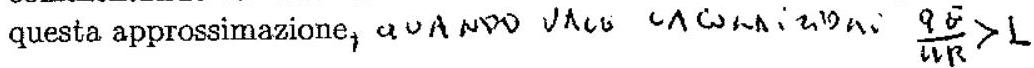
\includegraphics[max width=\textwidth]{2023_04_03_c2b519dab57738b76b16g-01}
\end{center}

\begin{enumerate}
  \setcounter{enumi}{3}
  \item assumendo \(k=0\), esaminare se sono possibili moti in cui \(O\) e allineato con l'asta.
\end{enumerate}

\begin{center}
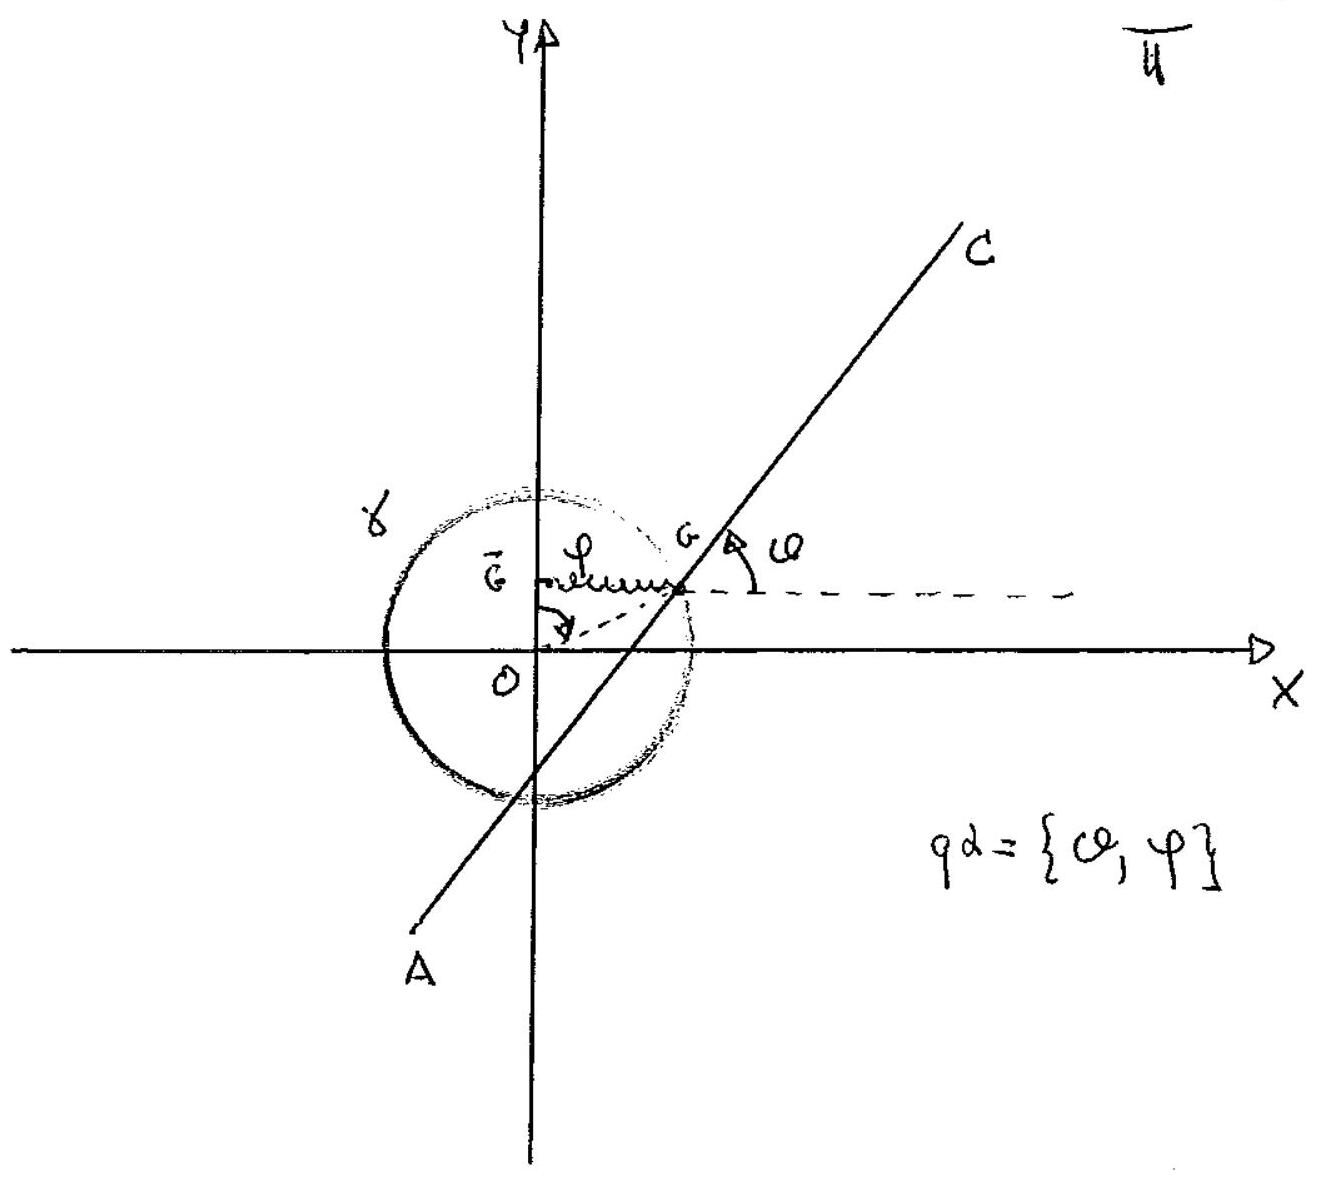
\includegraphics[max width=\textwidth]{2023_04_03_c2b519dab57738b76b16g-01(1)}
\end{center}

\section{Università degli studi di Catania
Corso di laurea Triennale in Fisica
Prova in itinexe per il corso di Meccanica Analitica
Appello del 29.04.2016}
In un piano verticale II è posto un sistema materiale è costituito da due punti \(P_{1}\) e \(P_{2}\) di uguale massa \(m\), vincolati a muoversi rispettivamente su due circonferenze \(C_{1}\) e \(C_{2}\) di uguale raggio \(R\), con i centri \(O_{1}\) ed \(O_{2}\) posti a distanza \(4 R\). Sui due punti \(P_{1}\) e \(P_{2}\) agiscono le forze

\[
\left\{F_{1}=-k\left(P_{1}-P_{2}\right), P_{1}\right\}, \quad\left\{F_{2}=-k\left(P_{2}-P_{1}\right), P_{2}\right\}
\]

dove \(k>0 . \Pi\) piano \(\Pi\) é posto in rotazione uniforme, con velocitá angolare \(\omega\), attorno alla retta \(\mathrm{r}\) di \(\Pi\) perpendicolare, al segmento \(\bar{O}_{1} O_{2}\), nel punto medio tra \(O_{1}\) ed \(O_{2}\). Tutti i vincoli sono realizzati senza attrito. Si chiede di:

\begin{enumerate}
  \item Verificare che sono configurazioni di equilibrio per il sistema le 4 configurazioni per le quali \(P_{1}\) e \(P_{2}\) sono allineati con \(O_{1}\) ed \(O_{2}\) e studiare la stabilitá della configurazione \(S_{1}\) in cui i punti \(P_{1}\) e \(P_{2}\) hanno distanza minima.

  \item Determinare le condizioni sui parametri \(\omega\) e \(k\) affinché siano configurazioni di equilibrio quelle per cui i vettori \(P_{1}-O_{1}\) e \(P_{2}-O_{2}\) siano ortogonali ad \(O_{1}-O_{2}\)

\end{enumerate}

Nelle condizioni di cui al punto 2.

\begin{itemize}
  \item Scrivere le equazioni di moto del sistema e gli eventuali integrali primi.

  \item Studiare le equazioni in prima approssimazione attorno alla configurazione di equilibrio \(S_{1}\).

  \item Verificare se esistono moti per \(i\) quali i vettori \(P_{1}-O_{1}\) e \(P_{2}-O_{2}\) si mantengono paralleli, ed in tali condizioni dire di che moto si tratta.

\end{itemize}

\begin{center}
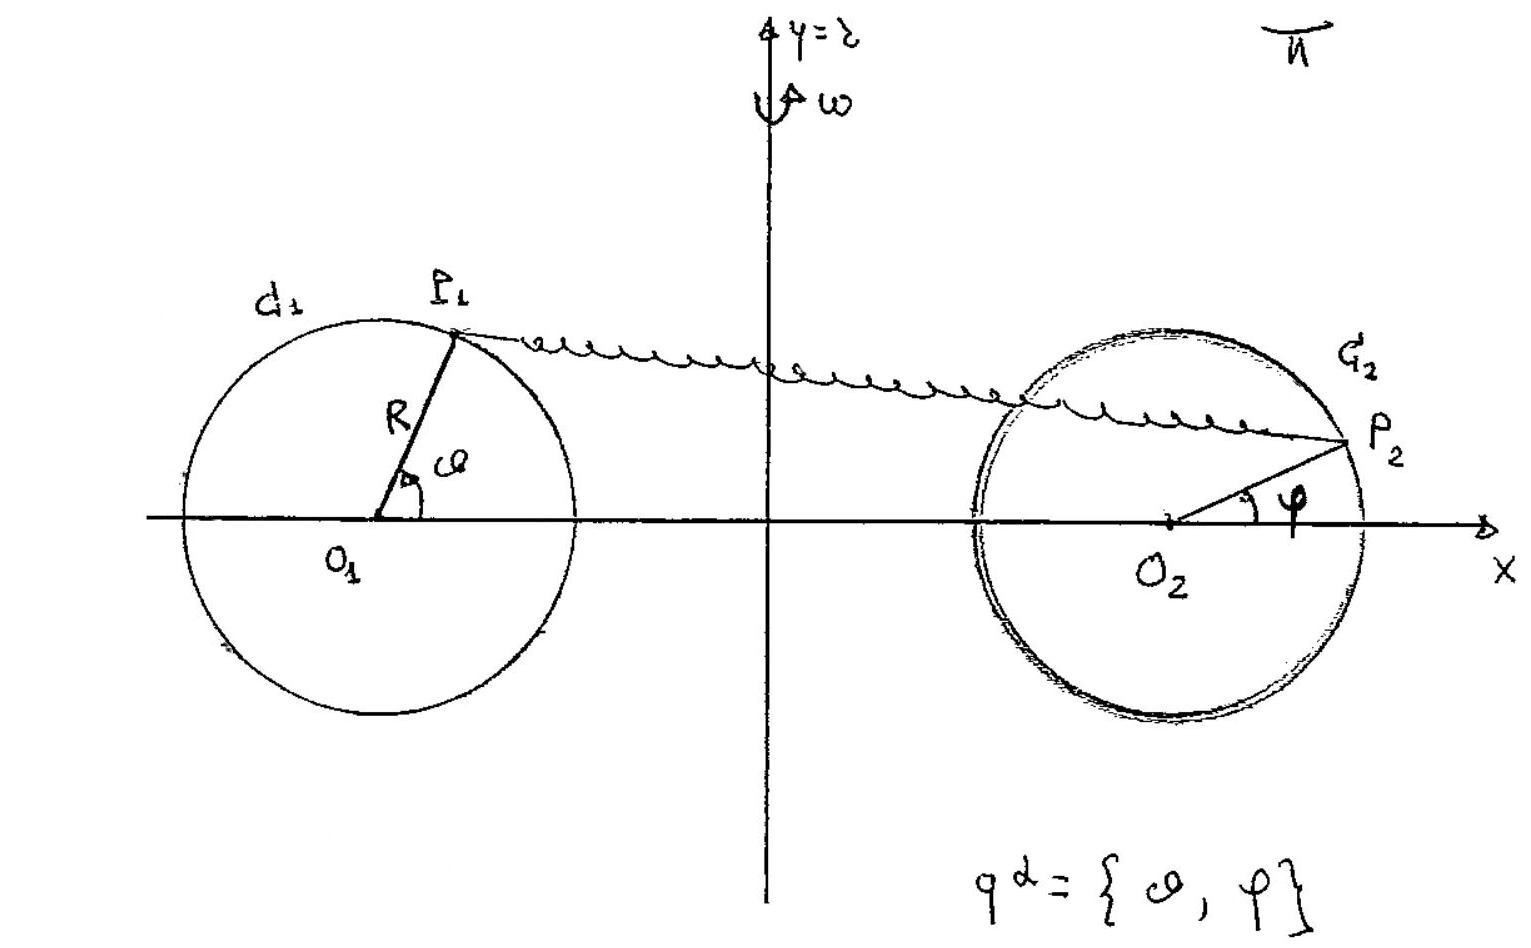
\includegraphics[max width=\textwidth]{2023_04_03_c2b519dab57738b76b16g-02}
\end{center}

\section{Università degli studi di Catania
Corso di laurea Triennale in Matematica
Prova in itinere per il corso di Fisica Matematica
Appello del 20.04.2016}
In un piano verticale \(I\) sono poste due guide rettilinee ortogonali fisse \(s_{1}\) ed \(\mathbf{s}_{2}\), formanti un angolo di \(\pi / 4\) con la verticale \(\mathrm{r}\) passante per il punto comune \(o\). Un sistema materiale \(S\) costituito da due dischi omogenei \(\gamma_{1}\) e \(\gamma_{2}\), aventi rispettivamente centri \(G_{1}\) e \(G_{2}\) raggi \(r_{1}\) e \(r_{2}\) con \(r_{1}<r_{2}\) ed uguale massa \(M\), é vincolato senza attrito a stare su \(\Pi\), inoltre \(\gamma_{1}\) e \(\gamma_{2}\) sono vincolati a rotolare senza strisciare rispettivamente su \(s_{1}\) ed \(s_{2}\).

Sapendo che sul sistema oltre alla forza peso agiscono le forze

\[
\left\{F_{1}=-k\left(G_{1}-G_{2}\right), G_{1}\right\}, \quad\left\{F_{2}=-k\left(G_{2}-G_{1}\right), G_{2}\right\}
\]

dove \(k>0\) e che il piano \(\Pi\) é posto in rotazione uniforme (con velocitá angolare \(\Omega\) ) attorno ad \(r\), si chiede di determinare al variare del parametro \(k\) :

\begin{enumerate}
  \item le eventuali configurazioni di equilibrio e discuterne la stabilitá.

  \item scrivere le equazioni di moto, e gli eventuali integrali primi.

  \item studiare il moto del sistema al variare di \(k\);

  \item determinare sotto quali condizioni sui parametri, e con quali condizioni iniziali, si possono avere moti in cui \(\gamma_{1}\) sta in quiete.

\end{enumerate}

\begin{center}
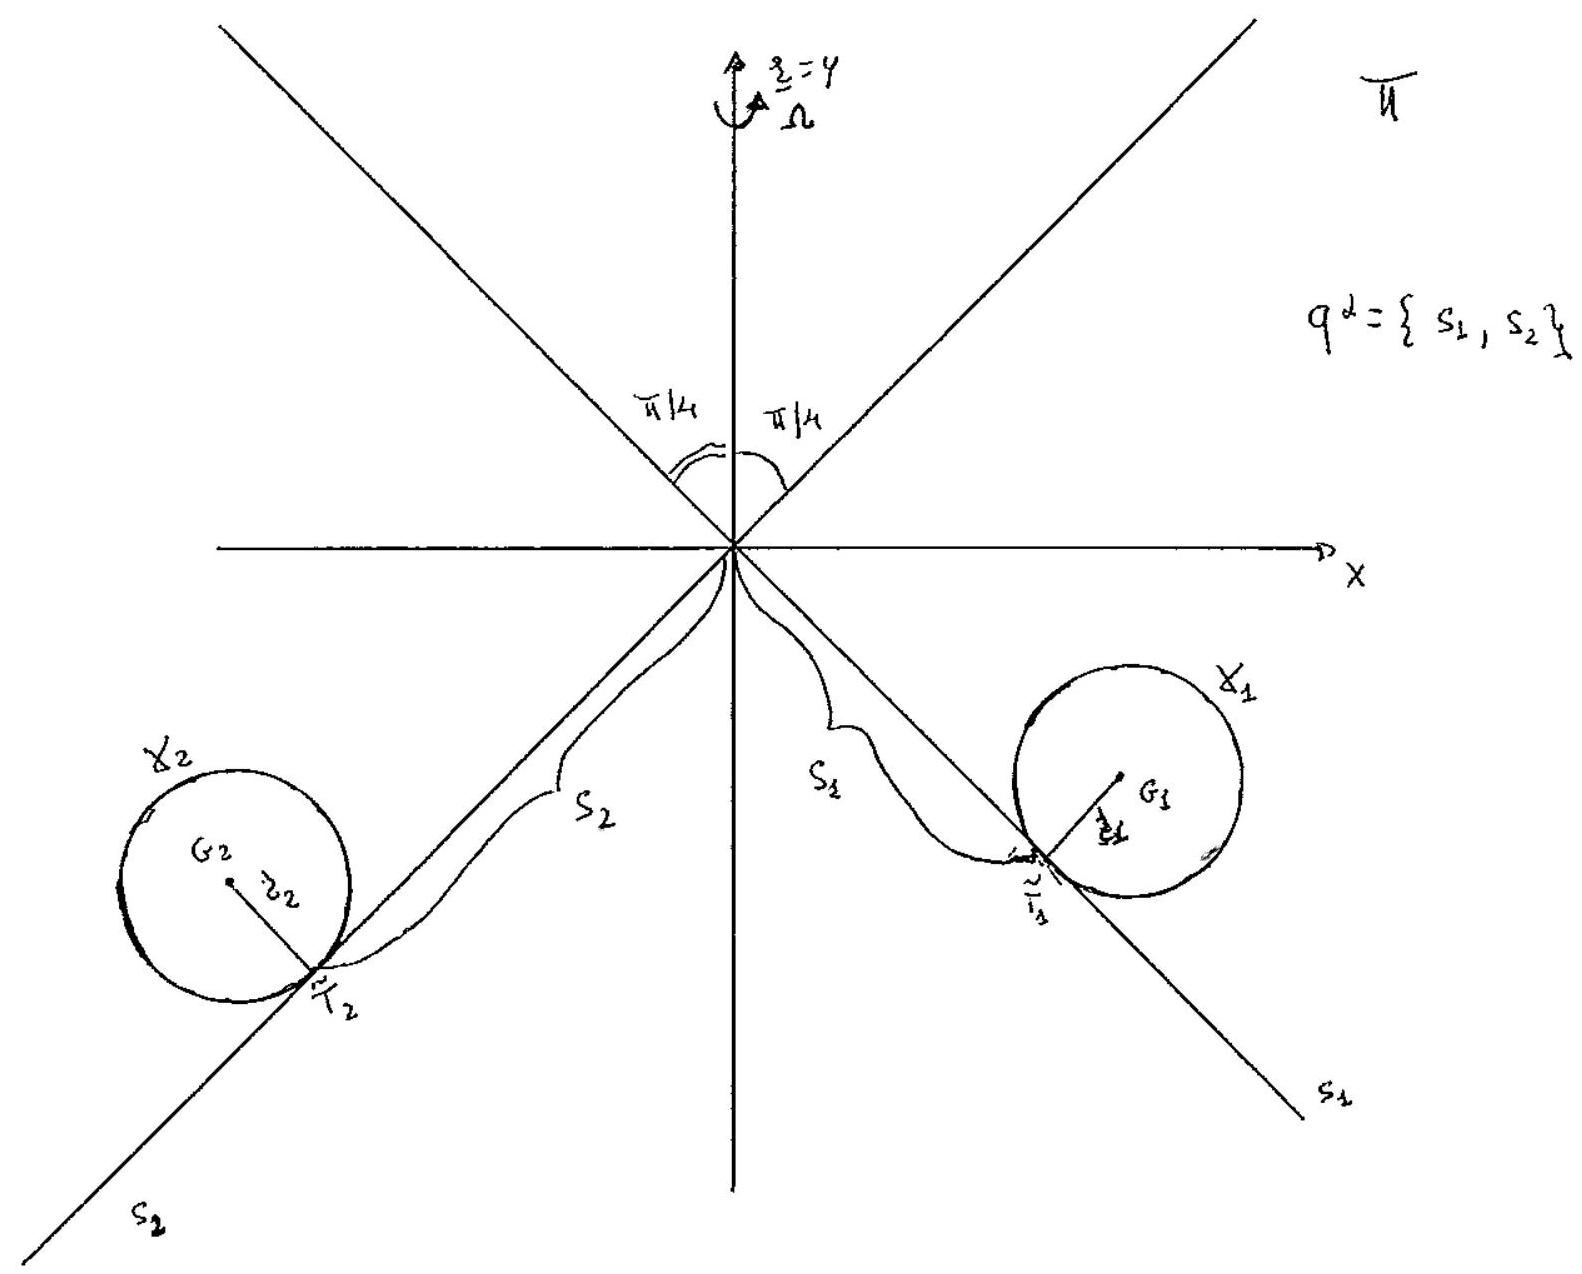
\includegraphics[max width=\textwidth]{2023_04_03_c2b519dab57738b76b16g-03}
\end{center}

\section{Università degli studi di Catania
Corso di laurea in Fisica
Meccanica Analitica
Appello del 04.03.2016}
Su nu piano verticale \(\Pi\) liscio é vincolato a stare, durante tutto il suo moto, un sistema materiale \(S\) costituito da un disco omogeneo \(\Gamma\) di massa \(m\), centro \(P\) e raggio \(r\) e da una circonferenza omogenea \(\gamma\) di massa \(m\), centro \(C\) e raggio \(d=r+R\), avente due punti \(M\) ed \(N\), diametralmente opposti, vincolati a muoversi su una verticale \(s\) di \(\Pi\).

Introdotto un sistema di riferimento ortogonale \(\{O, x, y\}\) con l'asse \(x\) verticale discendente coincidente con la retta \(s\) in modo che diametro \(M N\) di \(\gamma\) scorre senza attrito sull'asse delle \(x\), mentre \(\Gamma\) rotola internamente su \(\gamma\), senza strisciare. Sul sistema, oltre alle forze peso agisce l'ulteriore forza

\[
\left\{F=-\alpha \frac{m g}{R}(P \rightarrow O), P\right\}
\]

essendo \(O\) un punto fisso di \(s\) coincidente con l'origine del nostro riferimento, ed \(\alpha\) un numero reale positivo con \(\alpha \neq 1\).

Si chiede di:

\begin{enumerate}
  \item Determinare le configurazioni di equilibrio del sistema, e studiarne, ove possibile, la stabilitá al variare del parametro \(\alpha\).

  \item Determinare le equazioni di moto di \(S\) e gli eventuali integrali primi.

  \item Studiare i moti linearizzati attorno alla configurazione di equilibrio in cui \(P\) sta su \(s\) al di sotto di \(C\).

\end{enumerate}

U

\begin{center}
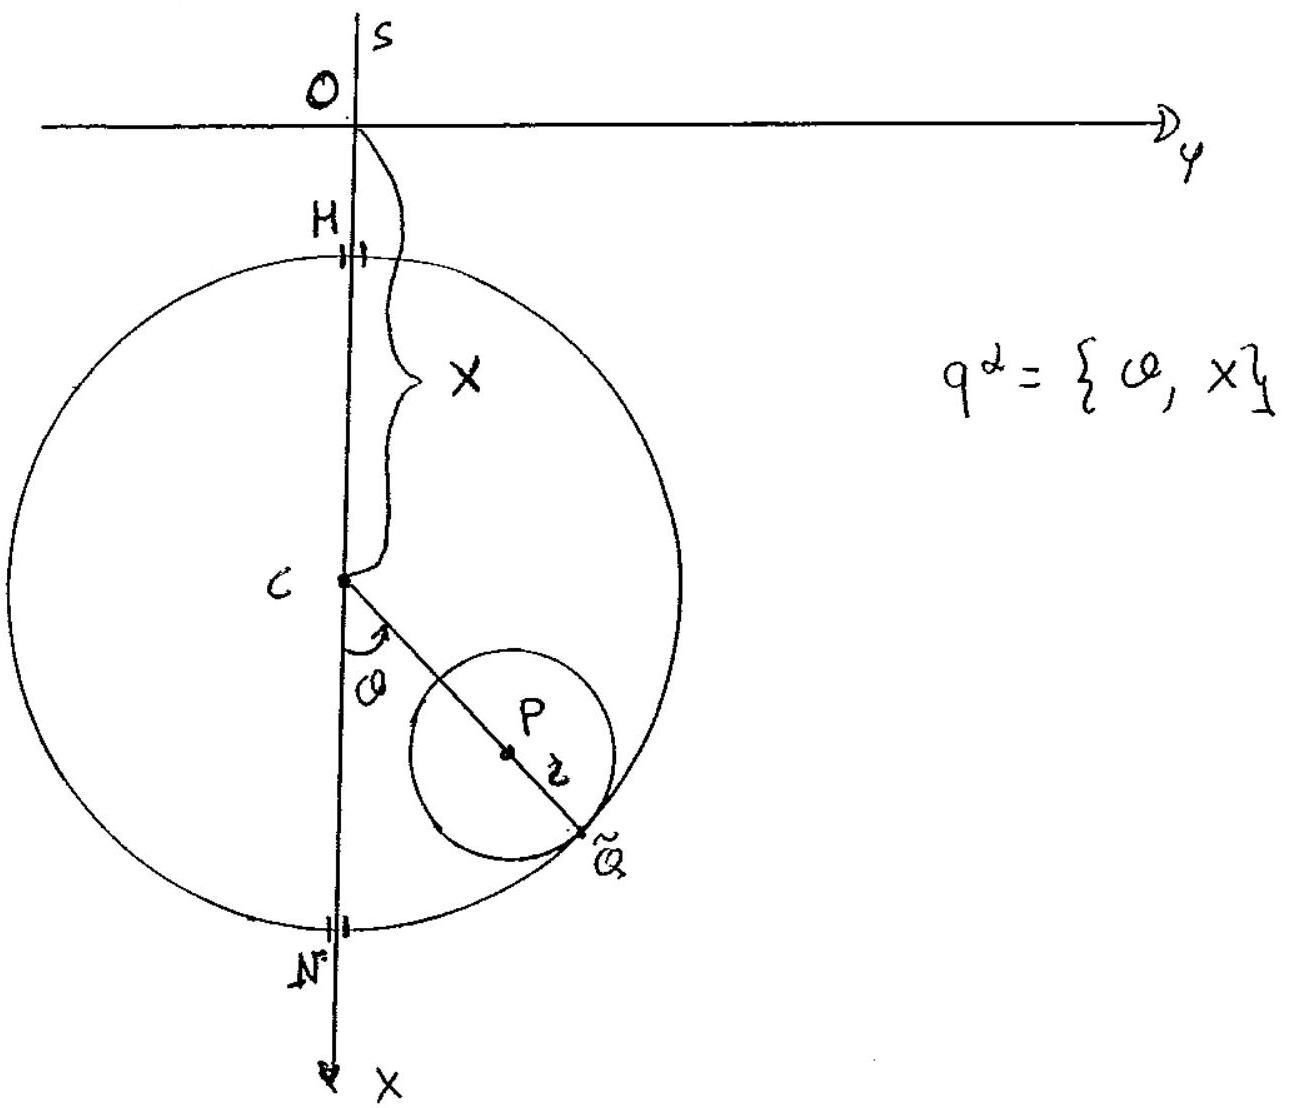
\includegraphics[max width=\textwidth]{2023_04_03_c2b519dab57738b76b16g-04}
\end{center}

\section{Università degli studi di Catania
Corso di laurea in Fisica
Compito di Meccanica Analitica
Appello del 12.02.2016}
Sia data una guida circolare \(\gamma\) di centro \(O\) e raggio \(R\) posta in un piano verticale II dove è stato introdotto un sistema di riferimento cartesiano ortogonale \(\{O, x, y\}\) con l'asse delle \(y\) verticale discendente. Un sistema materiale \(\mathrm{S}\) é costituito da due punti \(P\) e \(Q\) aventi la stessa massa \(m\), vincolati a muoversi senza attrito su \(\gamma\), ed é soggetto, oltre alla forza peso, alle due forze di mutua repulsione

\[
\{\mathrm{F}, P\} \quad \text { e } \quad\{-\mathrm{F}, Q\} \quad \text { con } \quad \mathbf{F}=4 \alpha m g R \frac{(P-Q)}{\mid P-Q\}^{2}}
\]

essendo \(\alpha\) una costante reale positiva.

Il sistema. ha ovviamente due gradi di libertá, scelte allora come coordinate Lagrangiane gli angoli \(\vartheta\) che \((P-O)\) forma con l'asse delle \(y\) e \(\psi\) che \((Q-O)\) forma con \((P-O)\) ambedue misurati in modo che le rotazioni di \(P\) per \(\vartheta\) crescente, e, per fissato \(P\), quella di \(Q\) per \(\psi\) crescente siano entrambe in senso antiorario.

\begin{enumerate}
  \item Dimostrare che la sollecitazione agente su \(S\) é conservativa e che per la coppia \(\{\vartheta, \psi\}\) delle due variabili lagrangiane \(0 \leq \vartheta \leq 2 \pi\) e \(0<\psi<2 \pi\)

  \item Determinare le configurazioni di equilibrio del sistema \(S\), studiando la stabilitá delle suddette configurazioni.

  \item Determinare le equazioni di moto e gli eventuali integrali primi.

  \item Studiare i moti linearizzati, determinando la frequenza dei piccoli moti, attorno ad una configurazione di equilibrio stabile.

\end{enumerate}

\begin{center}
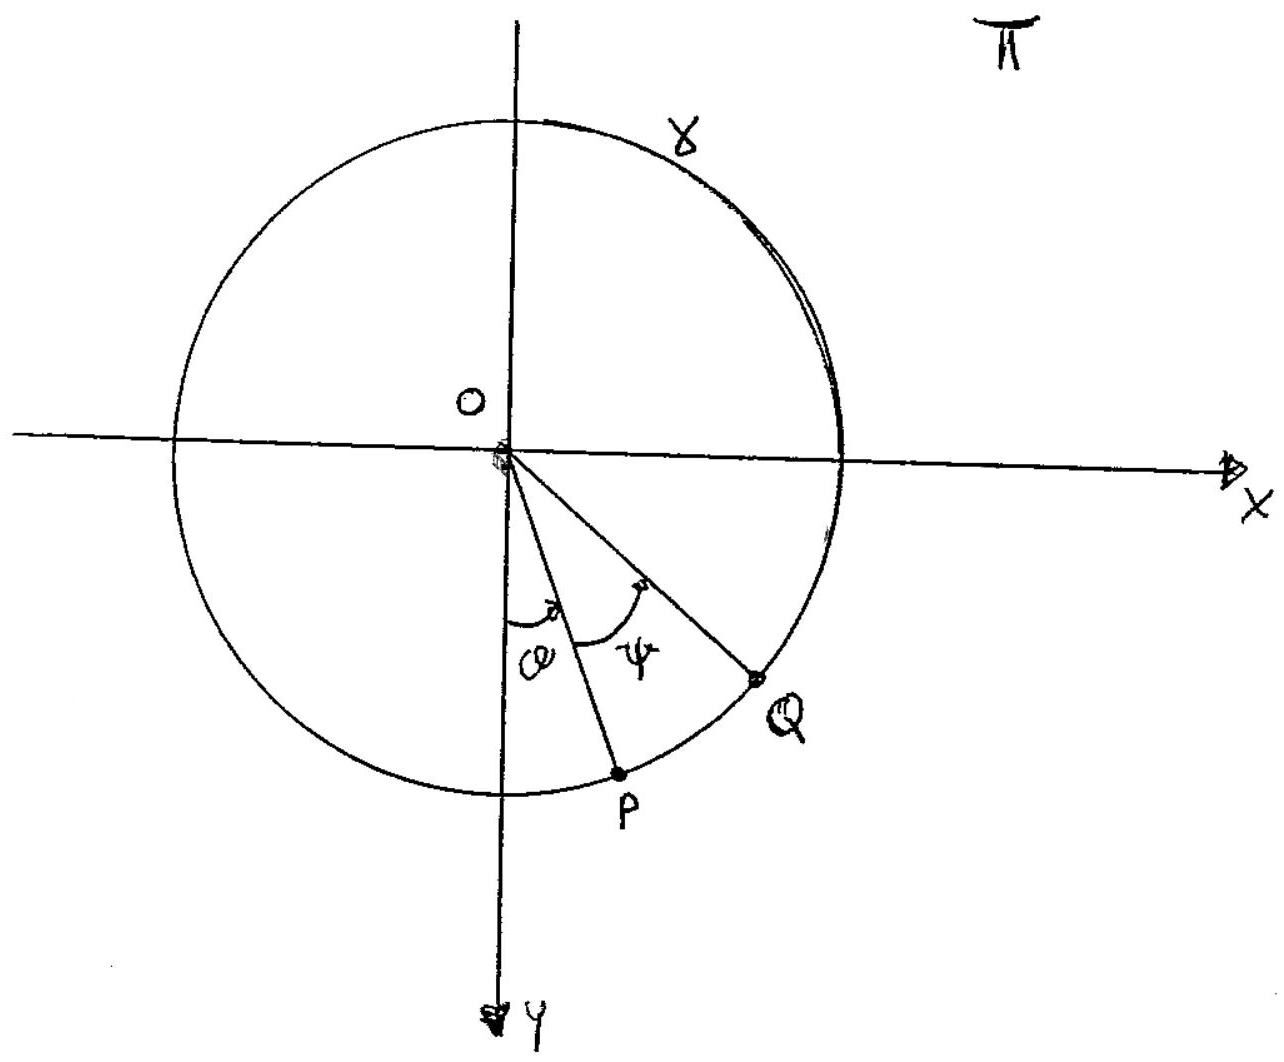
\includegraphics[max width=\textwidth]{2023_04_03_c2b519dab57738b76b16g-05}
\end{center}

\section{Università degli studi di Catania
Corsò di laurea in Matematica
Compito di Fisica Matematica
Appello' del 11.02.2016}
Sia dato un sistema materiale \(S\), posto in un piano verticale \(\Pi\), costituito dà una lamina quadrata \(O A B C\), omogenea e pesante, di massa \(m\) diagonale \(2 L\) e baricentro \(G\), e da un punto materiale \(P\) avente anch'esso massa \(m\), vincolato a scorrere senza attrito lungo la diagonale \(O B\) della lamina. La lamina quadrata. puó ruotare attorno al suo vertice \(O\) fisso nel piano verticale II. Oltre alle forze peso agiscono, sul punto materiale \(P\) e sul baricentro \(G\) della lamina quadrata, le seguenti forze elastiche

\[
\left\{F_{1}=-k(s-L) \frac{(P-O)}{|P-O|}, P\right\}, \quad\left\{F_{2}=-k(G-\bar{G}), G\right\},
\]

essendo s la distanza del punto \(P\) dal vertice \(O\) lungo la diagonale \(O B\) della lamina, la costante elastica \(k=\frac{2 m g}{L}\), e \(\vec{G}\) la proiezione del baricentro \(G\) della lamina, sulla verticale passante per \(O\). Supposti i vincoli lisci, e scegliendo come \(\{\vartheta, s\}\) le coordinate lagrangiane (si veda la figura), si chiede di determinare:

\begin{enumerate}
  \item Le configurazioni di equilibrio del sistema \(S\), indagando la stabilitá delle suddette configurazioni.

  \item Le equazioni di moto e gli eventuali integrali primi.

  \item I moti, in prima approssimazione, attorno alla configurazione di equilibrio in cui il sistema occupa la posizione corrispondente al piú piccolo valore di \(\vartheta\) consentito.

\end{enumerate}

\begin{center}
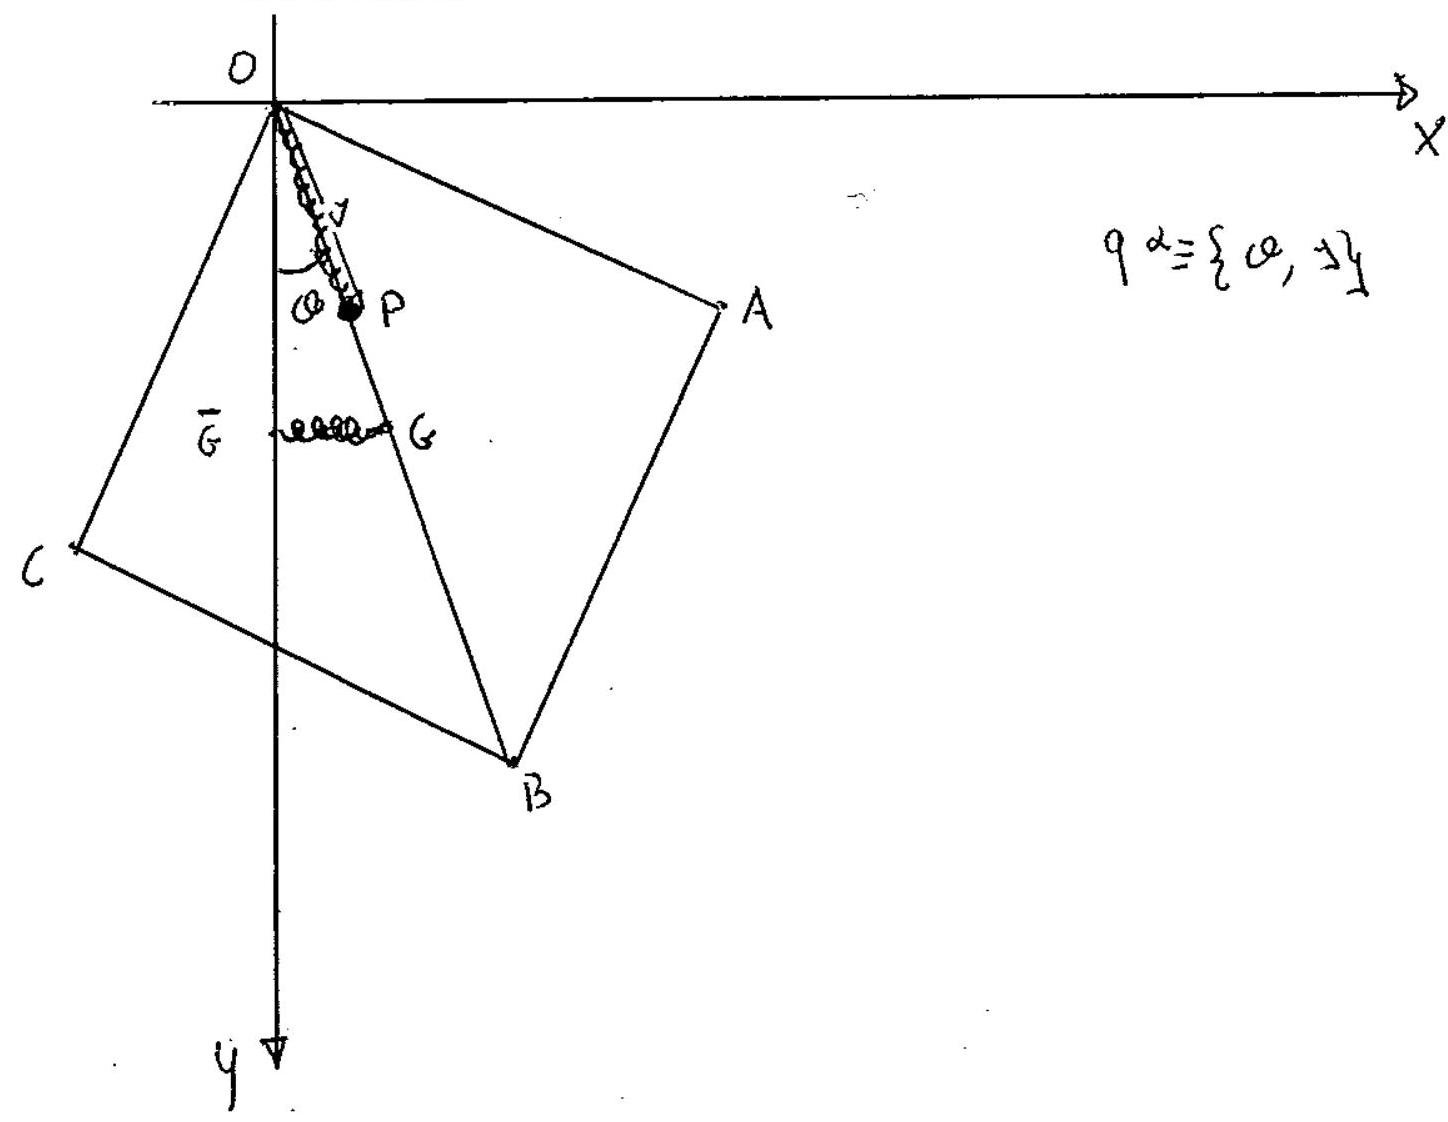
\includegraphics[max width=\textwidth]{2023_04_03_c2b519dab57738b76b16g-06}
\end{center}

\section{Università degli studi di Catania
Corso di laurea in Fisica
Compito di Meccanica Analitica Appello del 14.12.2015}
Un sistema materiale mobile \(S\), posto in un piano verticale, é costituito da due aste omogenee \(A B\) e \(C D\), aventi la stessa massa \(m\) e la stessa lunghezza 2l. Introdotto un sistema di riferimento cartesiano ortogonale \(\{O, \mathbf{i}, \mathbf{j}\}\) (come in figura), l'estremo \(A\) di \(A B\) é vincolato a muoversi su una guida verticale di equazione \(x=-d\), l'estremo \(C\) di \(C D\) é vincolato a muoversi su una guida verticale di equazione \(x=d\) (essendo \(2 d\) la distanza tra le due guide), mentre i secondi estremi \(B\) e \(D\) sono vincolati a muoversi su una guida sovrapposta all'asse delle \(X\). Supponendo che tutti i vincoli siano realizzati senza attrito e che sul sistema \(S\), oltre alla forza peso, agiscano le forze

\[
\left\{-\gamma\left(C_{1}-C_{2}\right), C_{1}\right\} \quad \text { e } \quad\left\{-\gamma\left(C_{2}-C_{1}\right), C_{2}\right\}
\]

e le due forze costanti

\[
\left\{-2 \gamma d i, C_{1}\right\} \quad \text { e } \quad\left\{2 \gamma d i, C_{2}\right\}
\]

essendo \(\gamma\) una costante positiva tale che \(\frac{m g}{2 \gamma l}>1\), e \(C_{1}, C_{2}\) rispettivamente i baricentri delle aste \(A B \cdot \mathrm{e} C D\).

\begin{enumerate}
  \item Determinare le configurazioni di equilibrio del sistema \(S\), analizzando la stabilitá delle suddette configurazioni.

  \item Determinare le equazioni di moto e gli eventuali iategrali primi.

  \item Studiare i moti linearizzati attorno alla configurazione di equilibrio nella quale le due aste occupano le posizioni piú basse.

  \item Determinare se esistono moti in cui le aste si mantengono parallele in ogni istante fra loro e, in caso affermativo, dare le condizioni iniziali per cui si verificano tali moti.

\end{enumerate}

\begin{center}
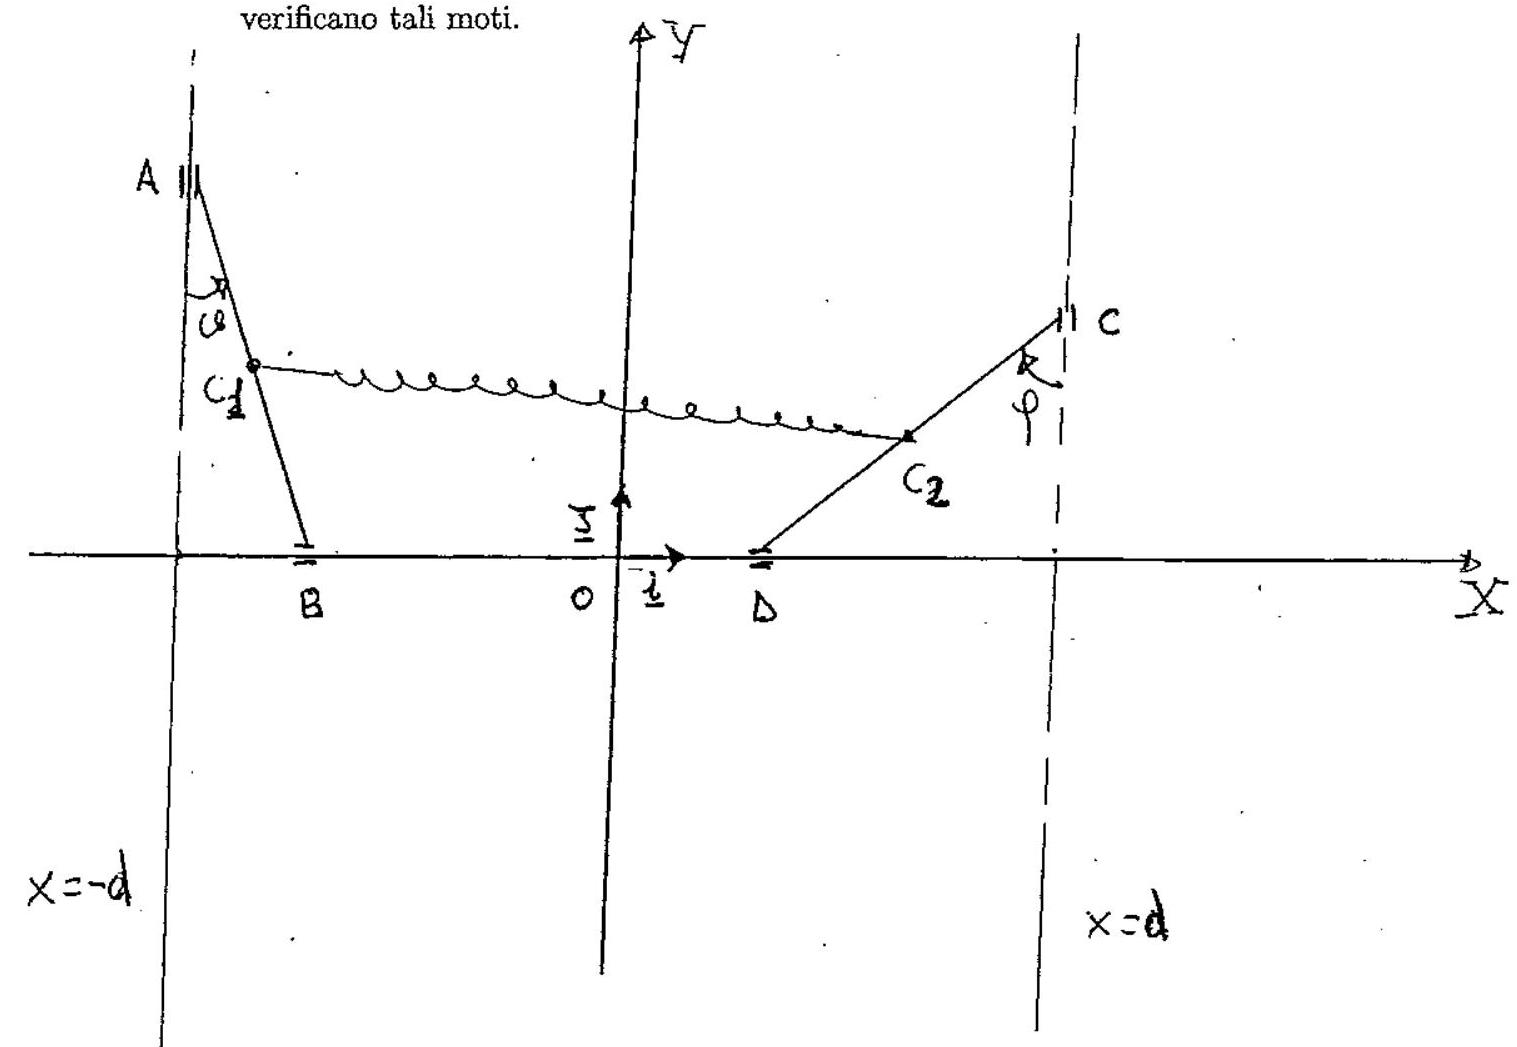
\includegraphics[max width=\textwidth]{2023_04_03_c2b519dab57738b76b16g-07}
\end{center}

\section{Università degli studi di Catania
Corso di laurea in Matematica
Compito di Fisica Matematica
Appello del 11.12.2015}
Sia dato un sistema materiale \(S\), costituito da un cilindro omogeneo di raggio \(R / 2\) altezza \(h\) e massa \(m\). L'asse del cilindro é vincolato a scorrere senza attrito, lungo l'asse \(Z\) di un sistema di riferimento ortonormale \(\{O, X, Y, Z\}\), tramite due cerniere cilindriche poste nei punti \(A\) e \(C\) rispettivamente in corrispondenza dei centri delle basi superiore ed inferiore del cilindro. Supposto che oltre alla forza peso sul sistema agiscano le forze elastiche

\(\left\{F_{1}=-2 \gamma(A-O), A\right\},\left\{F_{2}=-\sqrt{3} \gamma\left(B-A^{*}\right), B\right\},\left\{F_{3}=-\gamma(B-D), B\right\}\),

dove \(\gamma\) é una costante positiva, \(B\) é un punto posto sul bordo della base superiore del cilindro, \(A^{*}\) é la proiezione ortogonale di \(A\) su una retta verticale passante per l'asse \(X\) e distante \(R\) da \(Z, D\) é un punto sull'asse \(Y>0\) a distanza \(3 R\) dall'origine \(O\). Dati le coordinate Lagrangiani \(l=O A\) e \(\varphi=A^{*} \widehat{A} B\)

\begin{enumerate}
  \item Determinare le configurazioni di equilibrio del sistema \(S\), studiando lạ stabilitá delle suddette configurazioni.

  \item Determinare le equazioni di moto e gli eventuali integrali primi.

  \item Studiare i moti linearizzati attorno alle configurazioni di equilibrio.

\end{enumerate}

\begin{center}
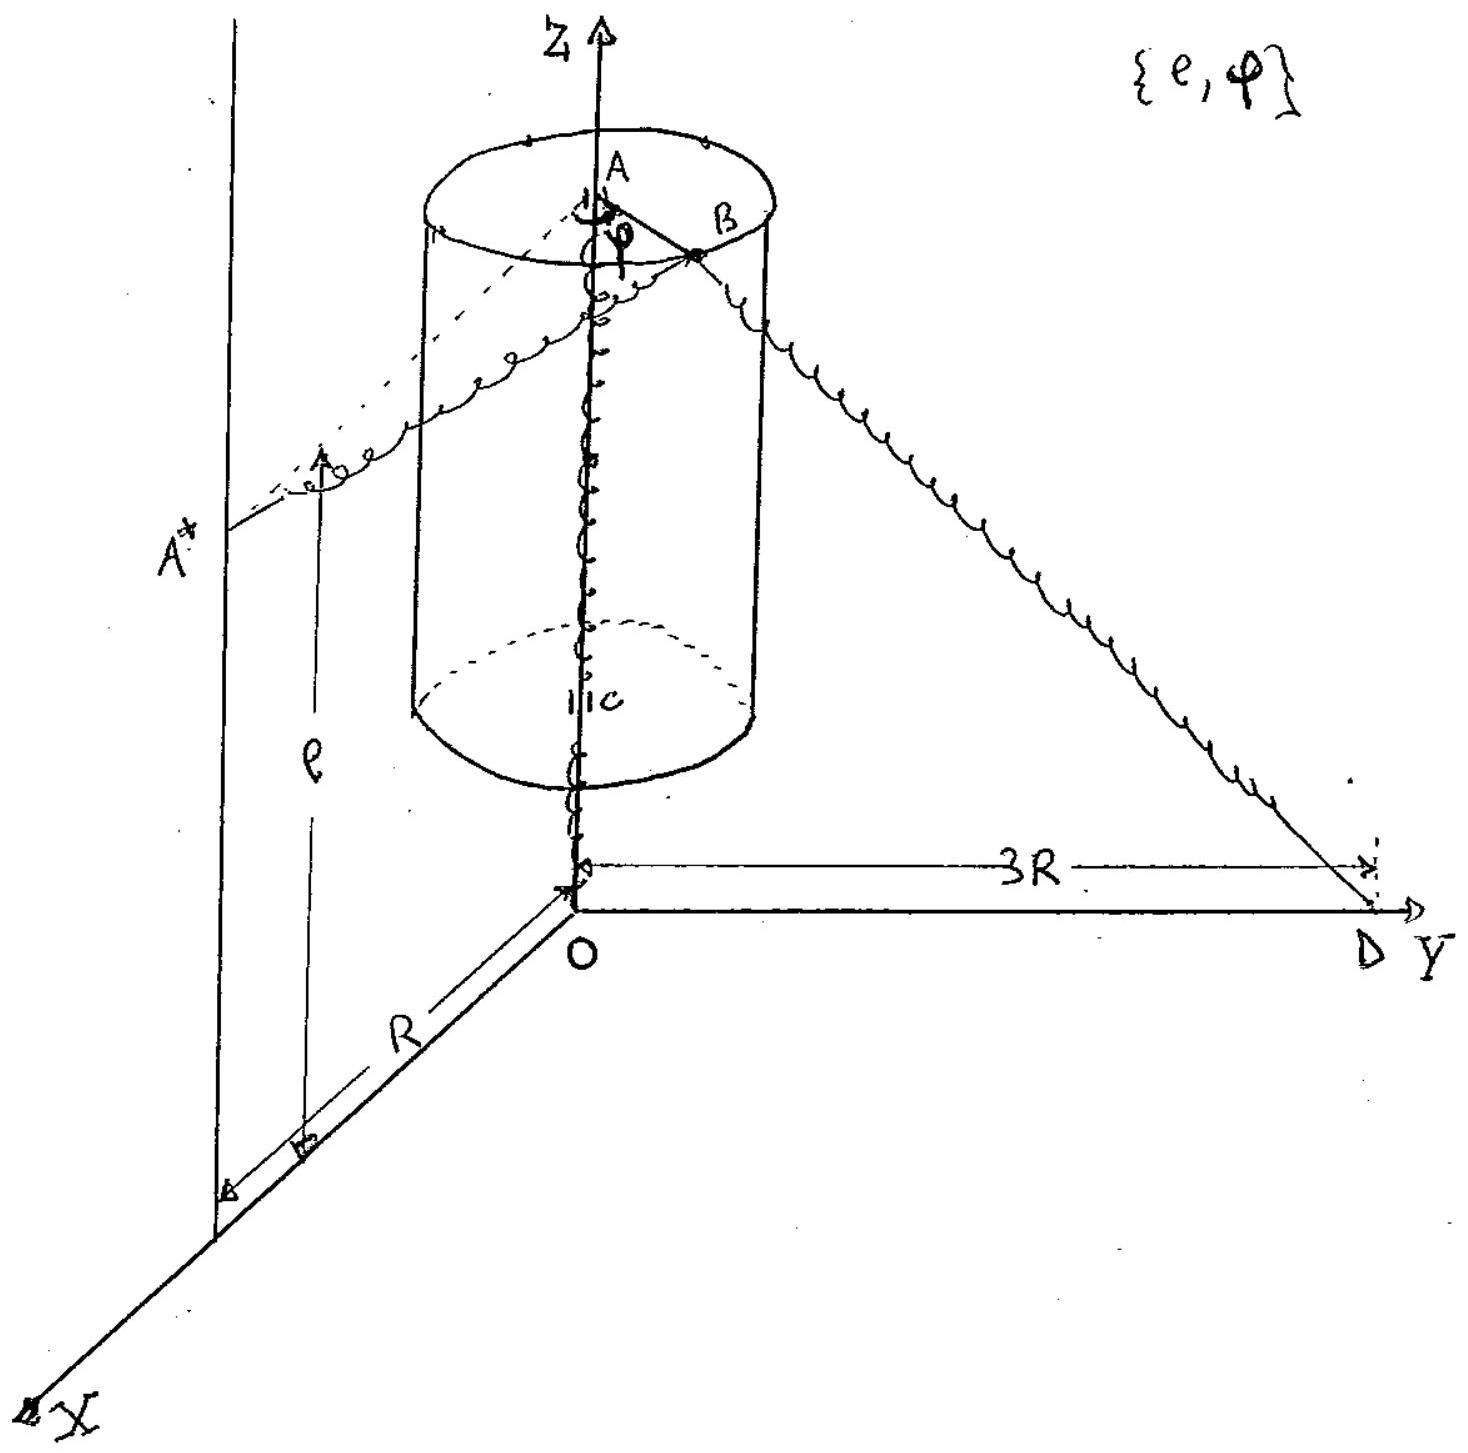
\includegraphics[max width=\textwidth]{2023_04_03_c2b519dab57738b76b16g-08}
\end{center}

\section{Università degli studi di Catania
Corso di laurea in Fisica
Meccanica Analitica
Appello del 03.10 .2014}
Un sistema materiale piano \(S\), mobile su un piano verticale \(\Pi\), é costituito da un disco omogeneo \(\Gamma\) di centro \(C\), raggio \(R\) e massa \(m\) e da un'asta omogenea \(A B\) di lunghezza \(4 L\) e massa \(m\), con l'estremo \(A\) inernierato al centro del disco. Tutti i precedenti vincoli sono realizzati senza attrito; inoltre il disco \(\Gamma\) é vincolato a rotolare senza strisciare su una guida orizzontale \(r\) di \(\ddot{\text { rimanendo }}\) superiormente ad essa. Sul sistema \(S\), oltre alle forze peso agiscono le forze

\[
\left\{-\frac{m g}{L}\left(C-C^{*}\right), C\right\}, \quad\left\{-\frac{m g}{L}\left(M-M^{*}\right), M\right\}
\]

essendo \(M\) il punto medio di \(A B, C^{*}\) ed \(M^{*}\) le proiezioni ortogonali di \(C\) ed \(M\) su una retta verticale \(s\) di \(\Pi\), e \(g\) il modulo dell'accelerazione di gravitá.

Supposto che il piano \(\Pi\) sia posto in rotazione uniforme attorno alla verticale \(s\) con velocitá angolare \(\omega=\sqrt{\alpha g / L}\) con \(0 \leq \alpha \leq 1\) si chiede, relativamente a \(\Pi\), di:

\begin{enumerate}
  \item determinare le configurazioni di equilibrio del sistema al variare di \(\alpha\), studiandone la stabilitá per \(0 \leq \alpha<1\)

  \item determinare le equazioni di moto e gli eventuali integrali primi (distinguendo il caso \(\alpha<1\) dal caso \(\alpha=1\) )

  \item studiare i moti linearizzati attorno alla evidente configurazione di equilibrio in cui l'asta \(A B\) é sovrapposta alla retta \(s\) con \(B\) al di sotto di A.

\end{enumerate}

\begin{center}
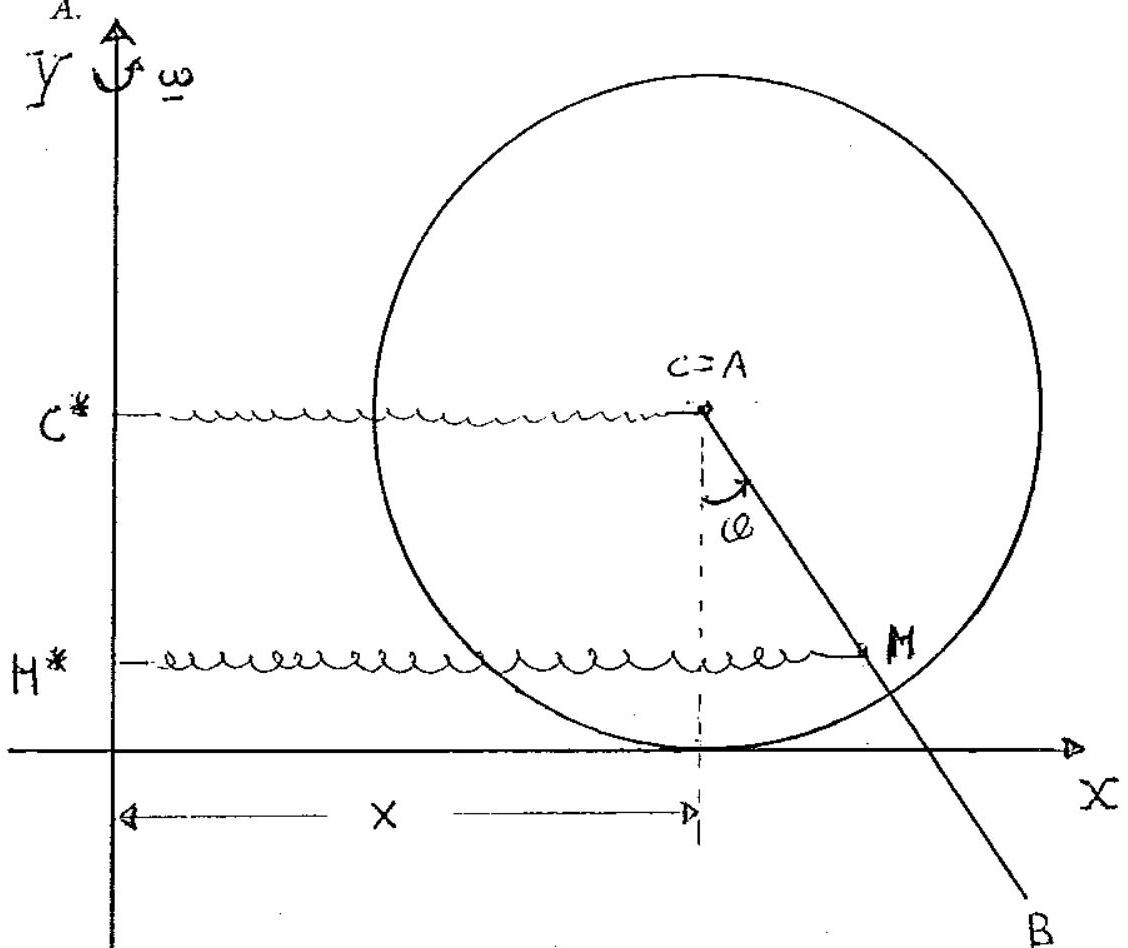
\includegraphics[max width=\textwidth]{2023_04_03_c2b519dab57738b76b16g-09}
\end{center}

\(B\)

\[
q^{\alpha} \geq\{x, e\}
\]

\section*{Università degli studi di Catania 
 Corso di laurea in Fisica 
 Meccanica Analitica 
 Appello del 12.09.2014 }
\textbackslash begin\{abstract\}
Un sistema materiale, costituito da due punti \(P\) e \(Q\) di uguale massa \(m\), é mobile su un piano verticale \(\Pi\). Il punto \(Q\) é vincolato a muoversi su una circonferenza \(\Gamma\) di \(\Pi\) di centro \(O\) e raggio \(R\), mentre \(P\) é vincolato a muoversi sulla retta orizzontale \(r\), tangente superiormente a \(\Gamma\).

Inoltre \(\Pi\) é in rotazione uniforme con velocitá angolare \(\underline{\omega}\) attorno alla verticale, appartenente a \(\Pi\), passante per il centro \(O\) di \(\Gamma\).

Supposto che tutti i vincoli siano realizzati senza attrito e che sui punti \(P\) e \(Q\), oltre alle forze peso, agiscano le forze

\[
\left\{-\frac{m g}{R}(P-O), P\right\}, \quad\left\{-\frac{m g}{R}(P-Q), P\right\}, \quad\left\{-\frac{m g}{R}(Q-P), Q\right\},
\]

essendo \(g\) l'accelerazione di gravitá, e, posto \(\psi^{2} \alpha g / R\) con \(\alpha \geq 0\) ed \(\alpha \neq 1+\sqrt{2}\), si chiede di:

\begin{enumerate}
  \item determinare le configurazioni di equilibrio relativo a \(I 1\) studiandone la stabilitá al variare di \(\alpha\);

  \item determinare le equazioni del moto relativo e gli eventuali integrali primi;

  \item studiare i moti linearizzati attorno ad una configurazione di equilibrio, che é stabile per opportuni valori di \(\alpha\), e confrontare la stabilitá lineare di tale configurazione con quella non lineare, al variare del parametro \(\alpha\).
\textbackslash end\{abstract\}

\end{enumerate}

\begin{center}
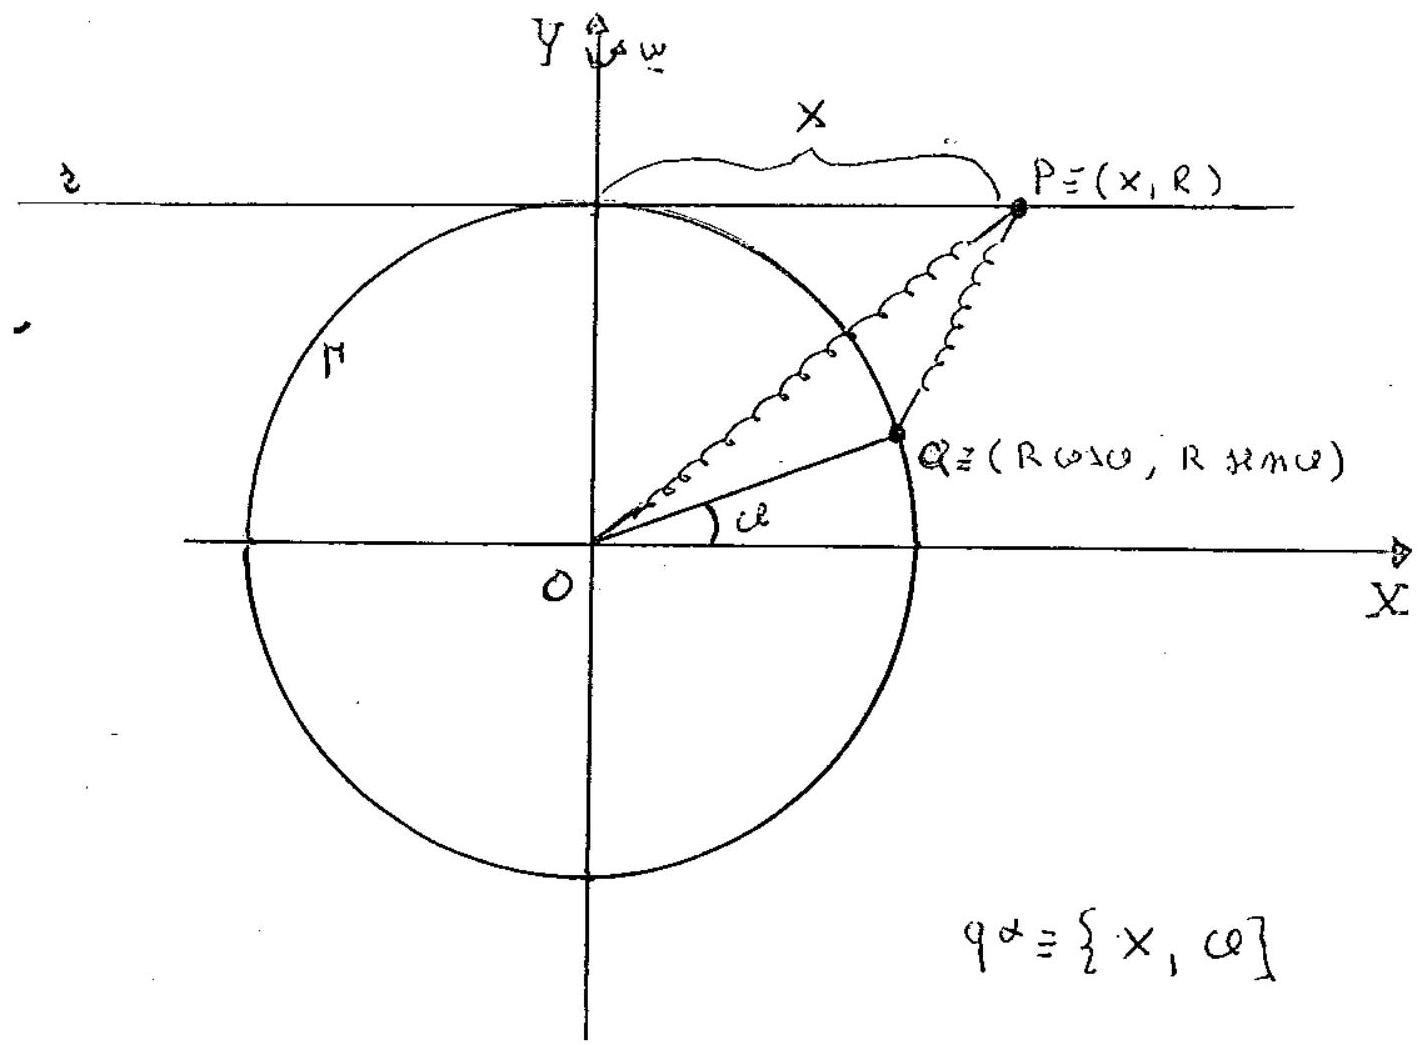
\includegraphics[max width=\textwidth]{2023_04_03_c2b519dab57738b76b16g-10}
\end{center}

\section{Università degli studi di Catania
Corso di laurea in Fisica
Meccanica Analitica
Appello del 18.07.2014}
Un sistema materiale, mobile su un piano verticale \(\Pi\), é costituito da un disco omogeneo \(\Gamma\) di centro \(C\), raggio \(R\) e massa \(M=2 m\) e da un bullone (da considerarsi puntiforme) di massa \(m\), saldato in un punto \(P\) di \(\Gamma\) (si indichi con \(d\) la distanza \(\overline{P C}\), con \(0 \leq d \leq R)\). Il centro \(C\) di \(\Gamma\) é vincolato a scorrere senza attrito su una retta orizzontale \(r\) di \(\pi\).

Sul sistema, oltre alle forze peso, agiscono le due forže '

\(\left\{F_{1}=-k\left(P-P^{*}\right), P\right\} \quad\left\{F_{2}=-h\left(B \quad B^{*}\right), B\right\} \quad\) con \(k>0, \quad h \geq 0\), essendo \(P^{*}\) la proiezione ortogonale di \(P\) su uha retta verticale \(s\) di \(\Pi, B\) l'intersezione del raggio di \(\Gamma\) contenente \(P\) con il bordo di \(\Gamma\) (un punto fissato del bordo di \(\Gamma\) nel caso \(d=0\) ), \(B^{*}\) la proiezione ortogonale di \(B\) su una guida orizzontale \(t\) di \(\Pi\), posta superiormente ad \(r\) e distante \(L\) da essa. Supponendo che i vincoli siano lisci, si chiede di

\begin{enumerate}
  \item determinare \(h\) in modo che esistano configurazioni dai equilibrio nelle quali \(B\) sta sulla retta \(r\).
\end{enumerate}

Nella ipotesi di cui al punto 1 , si chiede poi di:

\begin{enumerate}
  \setcounter{enumi}{1}
  \item determinare le configurazioni di equilibrio del sistema, distinguendo i casi \(d>0\) e \(d=0\), studiando in particolare la stabilitá nel caso \(d>0\);

  \item determinare le equazioni di moto e gli eventuali integrali primi (distinguendo i casi \(d>0\) e \(d=0\) );

  \item nel caso \(d>0\), studiare i moti linearizzati attorno ad una configurazione di equilibrio in cui \(P\) sta su \(r\);

  \item nel caso \(d=0\), studiare il moto del sistema.

\end{enumerate}

\begin{center}
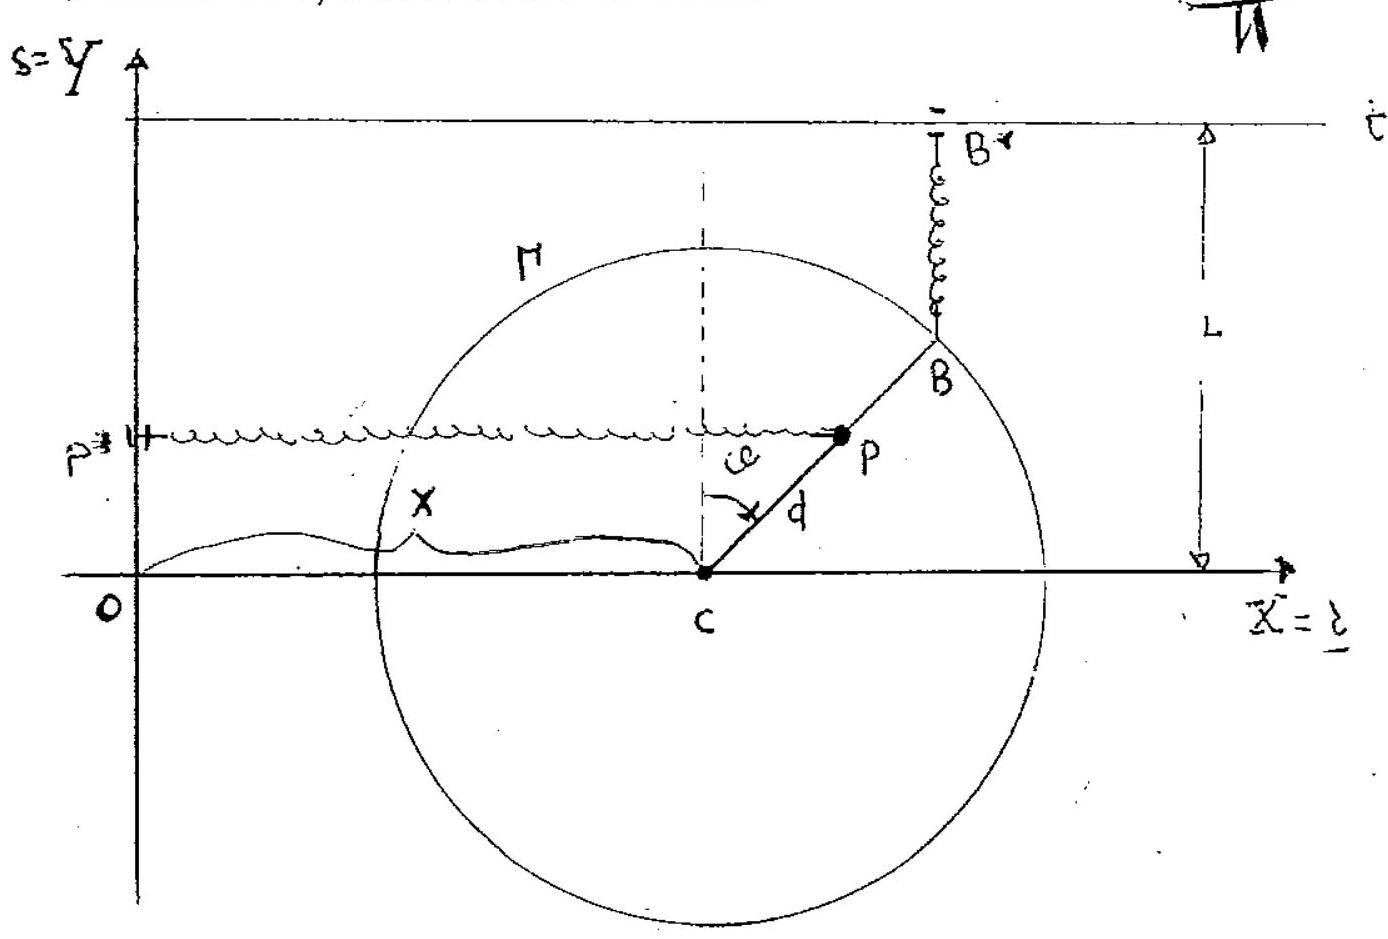
\includegraphics[max width=\textwidth]{2023_04_03_c2b519dab57738b76b16g-11}
\end{center}

\[
q^{\alpha}=(x, \theta)
\]

\section{Università degli studi di Catania
Corso di laurea in. Fisica
Meccanica Analitica
Appello del 27.06.2014}
Un sistema materiale é costituito da un disco omogeneo \(\Gamma\) di massa \(M\) centro \(G\) e raggio \(r\) e da una circonferenza omogenea \(\gamma\) di centro \(C\) e raggio \(R=r+d\) avente la stessa massa \(M\). Il sistema é vincolato a stare su un piano verticale II liscio, nel quale si é introdotto un sistema di riferimento ortogonale \(\{0, x, y\}\) con l'asse \(y\) verticale ascendente, ed é soggettonax seguenti vincoli: un diametro \(M N\) di \(\gamma\) scorre senza attrito sull'asse delle \(x\),mentre \(\dot{\Gamma} \cdot\) rótola internamente su \(\gamma\), senza strisciare.

Sul sistema, oltre alla forza peso \(M \mathrm{~g}\) agiscóno le vltertori forze

\[
\left\{F_{1}=-4 M \frac{g}{d}(G-\bar{G}), G\right\} \quad\left\{F_{2}^{3}=-2 M \frac{g}{d}(H-\bar{H}), H\right\}
\]

essendo \(\bar{G}\) la proiezione ortogonale di \(G\) sull'asse \(y, H\) il punto della circonferenza \(\gamma\) di massima quota, mentre \(\bar{H}\) é la proiezione ortogonale di \(H\) sull'asse \(y\). Inoltre il piano II é posto in rotazione uniforme attorno alll'asse \(y\) con velocitá angolare \(\omega=\sqrt{\alpha g / d}\) essendo \(\alpha\) una costante reale con la condizione che \(2<\alpha<3\) ed \(\alpha \neq 4-\sqrt{2}\). Si chiede di:

\begin{enumerate}
  \item Determinare le configurazioni di equilibrio del sistema, studiando in particolare la stabilitá della evidente configurazione di equilibrio \(S_{1}\), in cui \(C\) e \(G\) hanno coordinate rispettivamente \(C=(0,0)\) e \(G=(0,-d)\).

  \item Determinare le equazioni di moto e gli eventuali integrali primi.

  \item Studiare i moti linearizzati attorno alla configurazione di equilibrio \(S_{1}\) confrontando i risultati ottenuti con la stabilitá di \(S_{1}\)

\end{enumerate}

\begin{center}
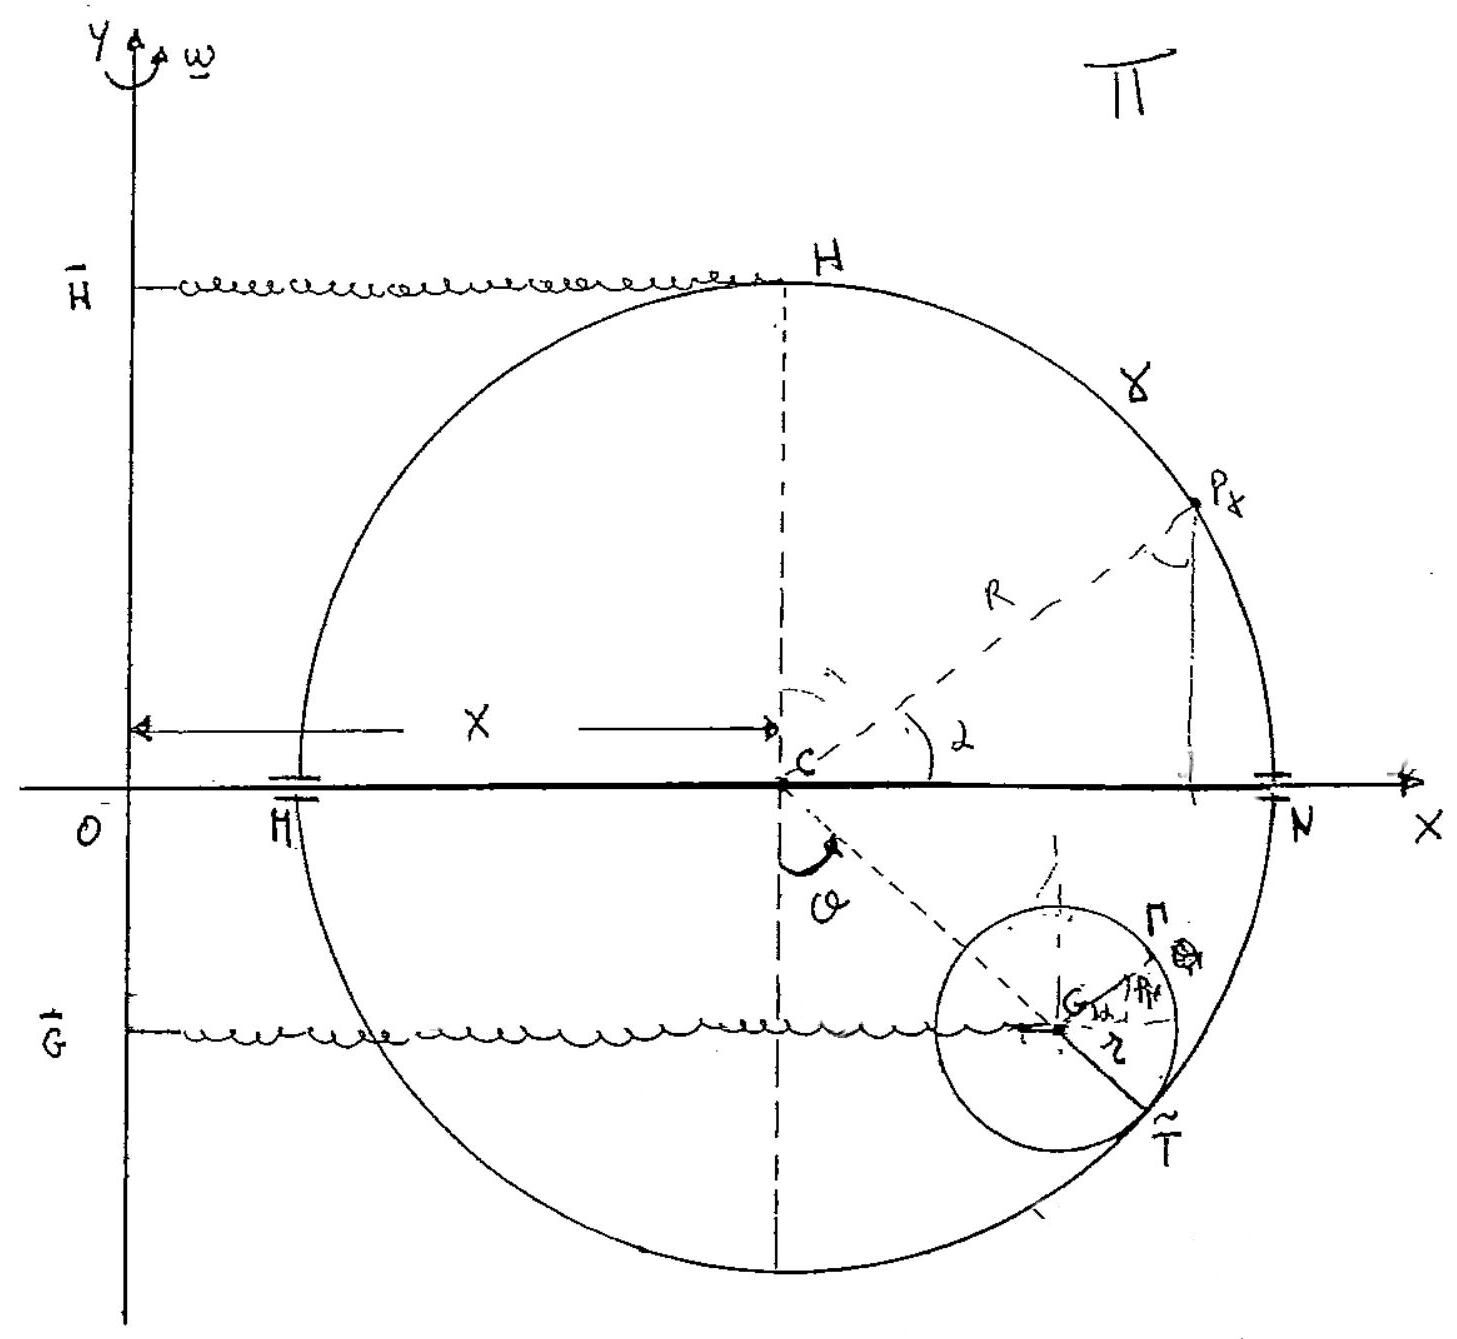
\includegraphics[max width=\textwidth]{2023_04_03_c2b519dab57738b76b16g-12}
\end{center}

\section{Università degli studi di Catania
Corso di laurea in Fisica
Meccanica Analitica
Appello del 11.06.2014}
Uń sistema materiale, posto su un piano verticale \(\Pi\), é costituito da un disco omogeneo \(\gamma\) di massa \(M\) e raggio \(R\) e da un'asta omogenea \(A B\) di massa \(2 M\) e lunghezza \(\sqrt{3} R\). Il sistema é soggetto ai seguenti vincoli: \(\gamma\) é vincolata a rotolare senza strisciare all'interno di una circonferenza fissa \(\Gamma\) di raggio \(2 R\); l'asta \(A B\) ha i suoi estremi \(A\) e \(B\) vincolati a scorrere senza attrito sul bordo di \(\gamma\).

Nell'ipotesi in cui, oltre alla forza peso, agisca la forza \(F=-k\left(C-C^{*}\right)\) applicata nel centro \(C\) di \(\gamma\), dove \(C^{*}\) é la proiezione ortogonale di \(C\) sulla retta fissa verticale passante per il centro \(O\) di \(\Gamma\) e supponendo che \(k>0\) con \(\frac{3 M g}{k R} \neq 1\), si chiede di:

\begin{enumerate}
  \item Determinare le configurazioni di equilibrio del sistema, indagando la stabilitá delle suddette configurazioni.

  \item Determinare le equazioni di moto e gli eventuali integrali primi.

  \item Studiare i moti linearizzati attorno alla configurazione di equilibrio nella quale il sistẹma occupa la posizione piú bassa consentita dai vincoli.

\end{enumerate}

\begin{center}
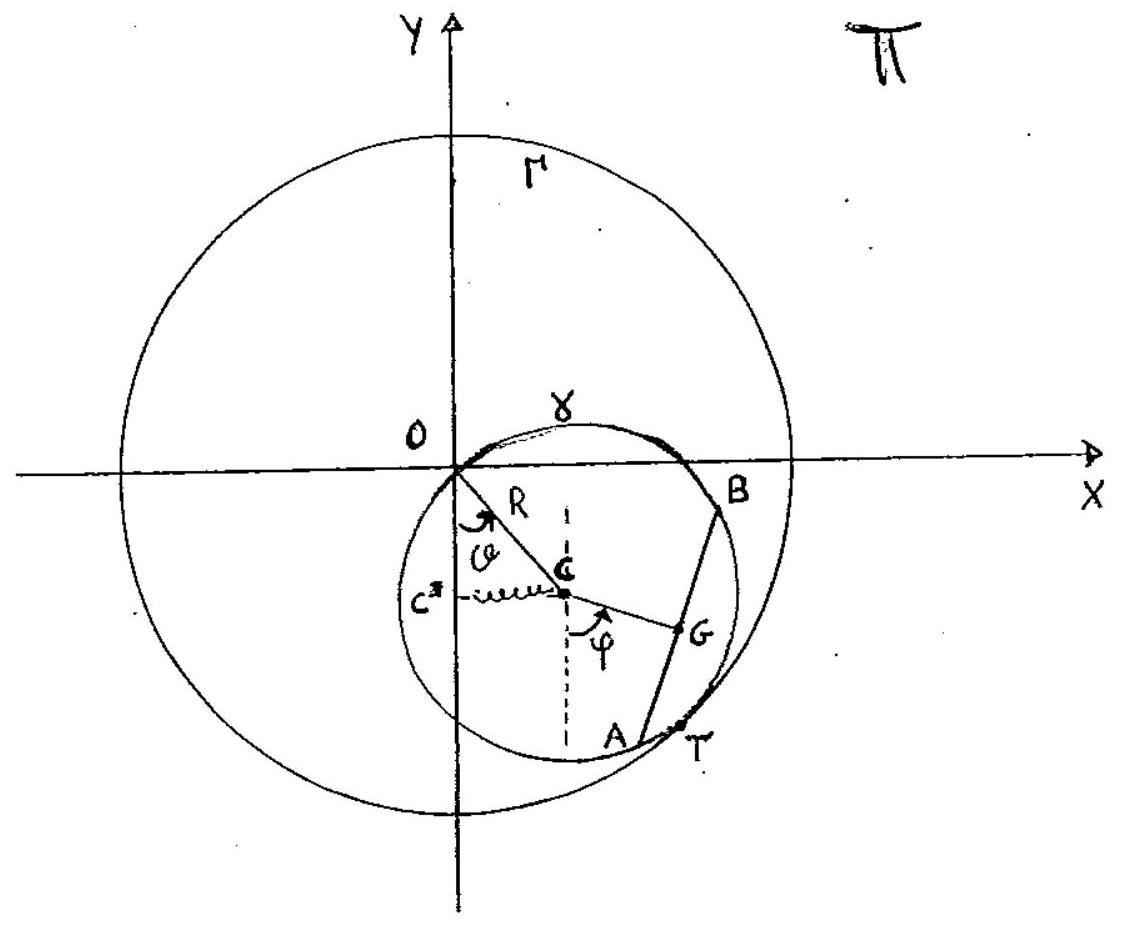
\includegraphics[max width=\textwidth]{2023_04_03_c2b519dab57738b76b16g-13}
\end{center}

\[
q^{\alpha} \equiv\{\vartheta, \varphi\}
\]

\section{Università degli studi di Catania
Corso di lauréa in Fisica
Meccanica Analitica
Appello del 19.05.2014}
Un sistema materiale, mobile in un piano verticale \(\Sigma\), é costituito da un'asta omogenea di massa \(m\) e lunghezza \(L\), avente un suo estremo \(A\) incerniato nel centro di un disco omogeneo di massa \(M\) e raggio \(R\), il quale é vincolato a rotolare senza strisciare su una guida orizzontale. Oltre alla forza peso agente sul sistema, sul punto \(A\) agisce una forza elastica \(F=-k(A-\bar{A})\) dove \(\bar{A}\) é la proiezione ortogonale di \(A\) su una retta fissa verticale.

Si chiede di:

\begin{enumerate}
  \item Determinare le configurazioni di equilibrio del sistema, indagando la stabilitá delle suddette configurazioni.

  \item Determinare le equazioni di moto e gli eventuali integrali primi.

  \item Studiare i moti linearizzati attorno alle configurazioni di equilibrio del sistema.

  \item Nell'ipotesi in cui \(k=0\) pronunziarsi sull'esistenza di altri integrali primi.

\end{enumerate}

\begin{center}
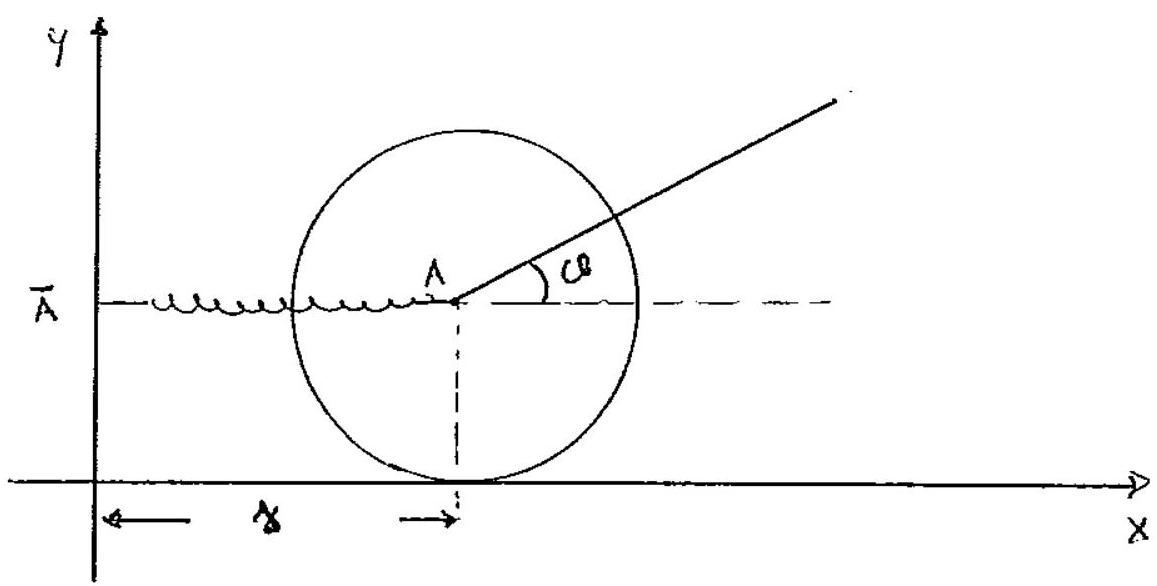
\includegraphics[max width=\textwidth]{2023_04_03_c2b519dab57738b76b16g-14}
\end{center}

\[
q \alpha \equiv\{\Delta, c\}
\]

\section{Università degli studi di Catania
Corso di laurea in Fisica
Meccanica Analitica
Appello del 03.03.2014}
Un sistema materiale, mobile in un piano verticale \(\Sigma\), é costituito da due aste omogenee \(\mathrm{PQ}\) e \(\mathrm{QR}\), aventi la stessa massa \(m\) e la stessa lunghezza \(2 L\), incerniate nel punto \(Q\). Introdotto un sistema di riferimento cartesiano ortogonale levogiro \(\{o, x, y, z\}\), avente il piano \(z=0\) sovrapposto al piano \(\Sigma\) e l'asse delle \(y\) verticale ascendente, si assuma che il punto medio \(M\) di \(P Q\) sia vincolato a muoversi sull'asse delle \(x\), mentre l'estremo \(R\) di \(Q R\) sia vincolato a muoversi sull'asse delle \(y\) e che tutti i vincoli siano realizzati senza attrito. Supposto che sul sistema, oltre alle forze peso, agisca la forza elastica

\[
\{F=-k(Q-\bar{Q}), Q\}
\]

essendo \(k=\frac{m g}{4 L \alpha}\) con \(\alpha>1, g\) il modulo della accelerazione di gravitá, e \(\bar{Q}\) la proiezione ortogonale di \(Q\) sull'asse delle \(y\). Si chiede di:

\begin{enumerate}
  \item Determinare le configurazioni di equilibrio del sistema, indagando la stabilitá delle suddette configurazioni.

  \item Determinare le equazioni di moto e gli eventuali integrali primi.

  \item Studiare i moti linearizzati attorno alla configurazione di equilibrio nella quale le due aste siano verticali e \(Q\) il punto piú basso del sistema

\end{enumerate}

\begin{center}
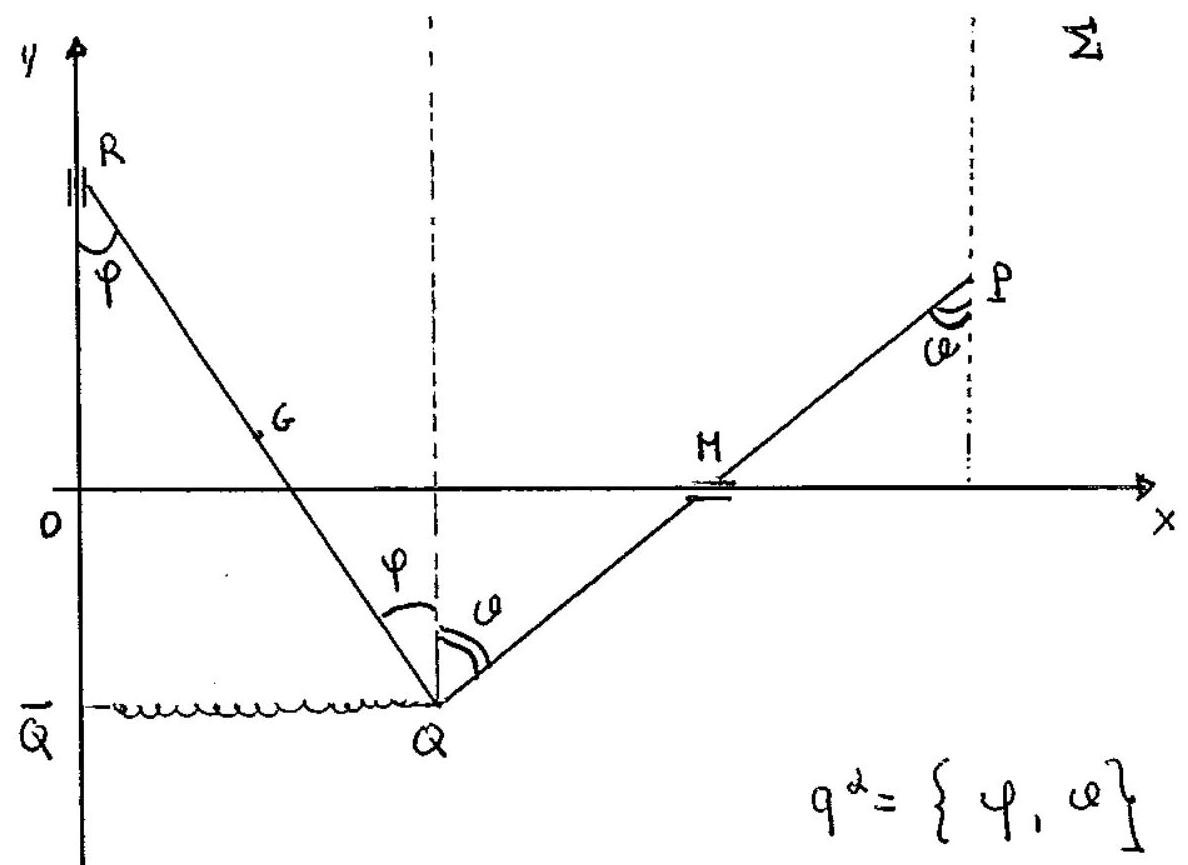
\includegraphics[max width=\textwidth]{2023_04_03_c2b519dab57738b76b16g-15}
\end{center}

\section{Università degli studi di Catania
Corso di laurea in Fisica
Meccanica Analitica
Appello del 20.11,2013}
Sia dato un sistema materiale \(S\) mobile, costituito da una circonferenza omogenea \(\gamma\) di massa \(m\) e raggio \(r\), vincolata a muoversi su un piano verticale \(\Pi\), mantenendo fisso un suo punto \(O\), e da un punto materiale \(P\) di uguale massa vincolato a muoversi su \(\gamma\). Supposto che oltre alla forza peso sul sistema agiscano le forze elastiche

\[
\left\{F_{1}=-\frac{m g}{2 R}(P-A), P\right\} \quad\left\{F_{2}=-\frac{m g}{2 R}(G-B), G\right\}
\]

essendo \(G\) ill centro di \(\gamma\), con \(A\) e \(B\) due punti nella verticale per \(O\) rispettivamente al di sopra ed al di sotto di \(O\) e a distanza \(2 R\) da esso. Supponendo che i vincoli siano lisci

!

Si chiede di:

\begin{enumerate}
  \item Determinare le configurazioni di equilibrio del sistema \({ }^{\prime} \mathrm{S}\), indagando la stabilitá delle suddette configurazioni.

  \item Determinare le equazioni di moto e gli eventuali integrali primi.

  \item Studiare i moti in prima approssimazione attorno alla evidente configurazione di equilibrio in cui \(G\) occupa la posizione piú bassa consentita dai vincoli e \(P\) coincida con \(B\).

\end{enumerate}

\begin{center}
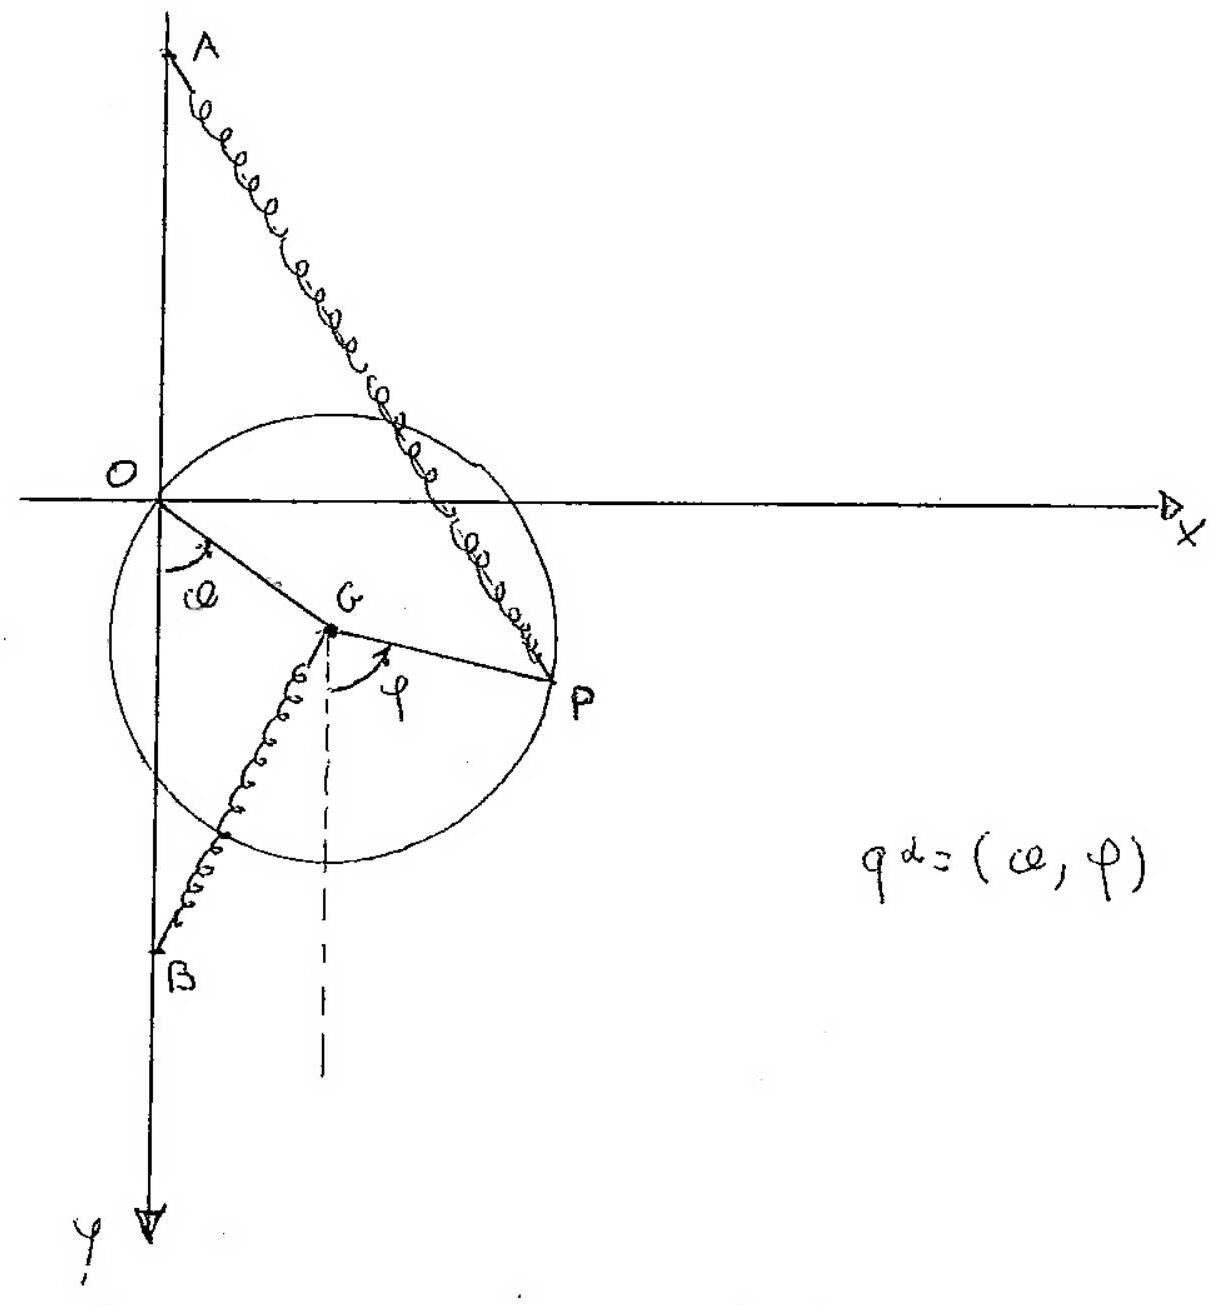
\includegraphics[max width=\textwidth]{2023_04_03_c2b519dab57738b76b16g-16}
\end{center}

\section{: Università degli studi di Catania
Corso di laurea in ingegneria civile ed ambientale
II Prova in itinere di Meccanica Razionale del \(13 / 06 / 2013\)}
Dato un sistema materiale \(S\), posto in un piano verticale \(\Pi\), costituito da un disco omogeneo \(\gamma\) di centro \(\mathrm{C}\), massa \(M\), raggio \(R=\sqrt{2} l\) con un buco circolare concentrico di raggio \(R / 2\) e da un'asta omogenea \(A B\) di lunghezza \(2 l\) avente la stessa massa \(M\). Il disco \(\gamma\) é vincolato a rotolare senza strisciare su una guida orizzontale \(r\) di \(\Pi\), mentre gli estremi A e B dell'asta sono vincolati a scorrere sul bordo di \(\gamma\). Sul sistema oltre alla forza peso, agisce la forza

\[
\{F=-k(G-\bar{G}), G\}
\]

essendo \(k>0, G\) il baricentro di \(A B\) e \(\bar{G}\) la sua proiezione ortogonale su una retta verticale \(s\) di \(\Pi\).

Supponendo \(i\) vincoli lisci si chiede di determinare:

\begin{enumerate}
  \item Le configurazioni di equilibrio del sistema \(S\), indagando la stabilitá delle suddette configurazioni.

  \item Le equazioni di moto e gli eventuali integrali primi. Inoltre nell'ipotesi in cui \(k=0\) pronunziarsi sull'esistenza di altri integrali primi.

  \item Studiare i piccoli moti attorno ad una configurazione di equilibrio stabile.

\end{enumerate}

\begin{center}
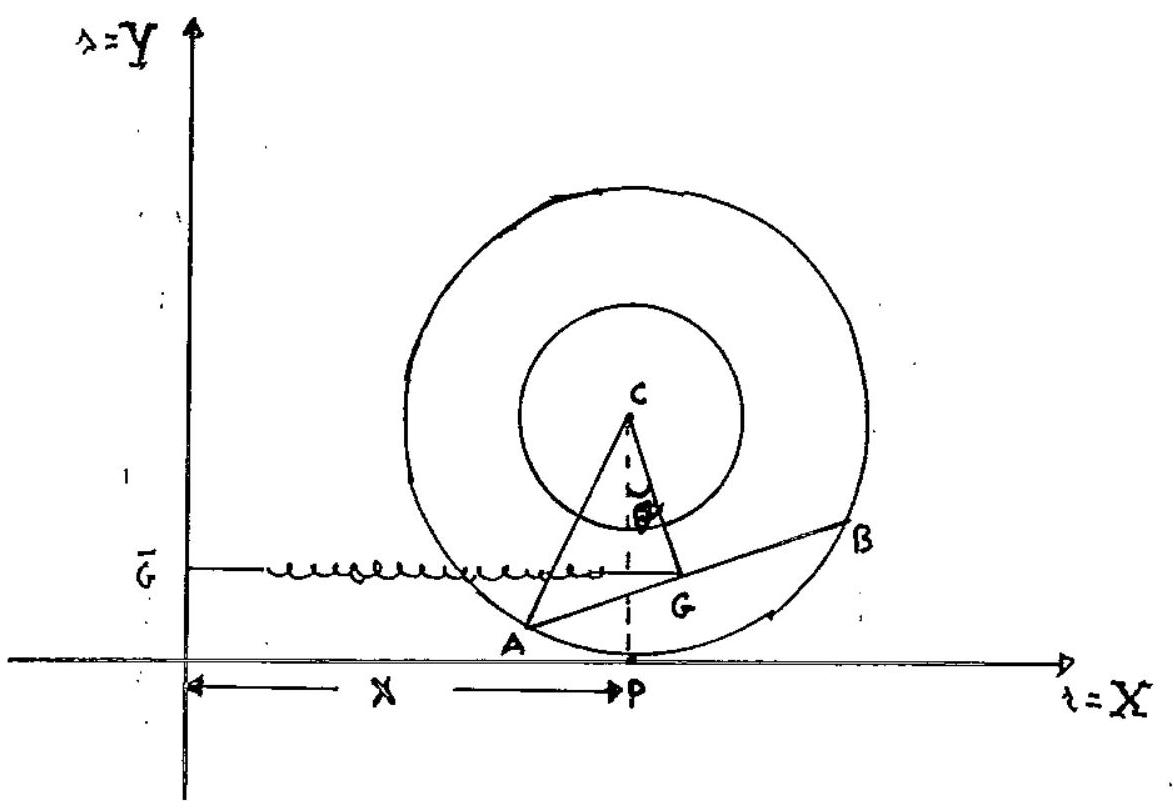
\includegraphics[max width=\textwidth]{2023_04_03_c2b519dab57738b76b16g-17}
\end{center}

\section{Università degli studi di Catania
Corso di laurea in ingegneria civile ed ambientale
Meccanica Razionale (Compito 2)
Appello del 24.06.2013}
Dato un sistema materiale \(S\) mobile in un piano verticale \(\Pi\) nel quale, introdotto un sistema di riferimento cartesiano ortogonale \(\{O, X, Y\}\) con l'asse delle \(Y\) verticale discendente, si trova una guida rettilinea \(\mathrm{r}\) di equazione \(y \Rightarrow R\), essendo \(R\) una fissata lunghezza. Il sistema \(S\) é costituito da un disco omogeneo \(\gamma\) di centro \(C\), raggio \(R\) e massa \(M\) e da un'asta omogenea di massa \(M\) e lunghezza \(2 L\), il cui estremo é incernierato in \(O\) e il cui secondo estremo indicheremo con A. Tutti i precedenti vincoli sono realizzati senza attrito, inoltre il disco \(\gamma\) é vincolato a rotolare senza strisciare sulla guida \(r\), in modo che il suo centro ha ordinata,' nel riferimento introdotto, costantemente nulla.

Sul sistema oltre alle forse peso, agiscono le due forze

\[
\{\dot{F}=-k(A-C), A\} \quad \text { e } \quad\{F=-k(C-A), C\}
\]

essendo \(k\) una opportuna costante positiva. Posto per semplicitá \(m g=4 \alpha k L\) essendo \(\alpha\) un numero reale positivo con \(\alpha \neq 1\), si chiede di determinare:

\begin{enumerate}
  \item Le configurazioni di equilibrio del sistema \(S\), indagando la stabilitá delle suddette configurazioni al variare di \(\alpha\).

  \item Le-equazioni di moto e gli eventuali integrali primi.

  \item Studiare i moti linearizzati attorno alla configurazione di equilibrio di \(S\) in cui il punto \(A\) occupa la configurazione piú bassa consentita dai vincoli.

\end{enumerate}

\begin{center}
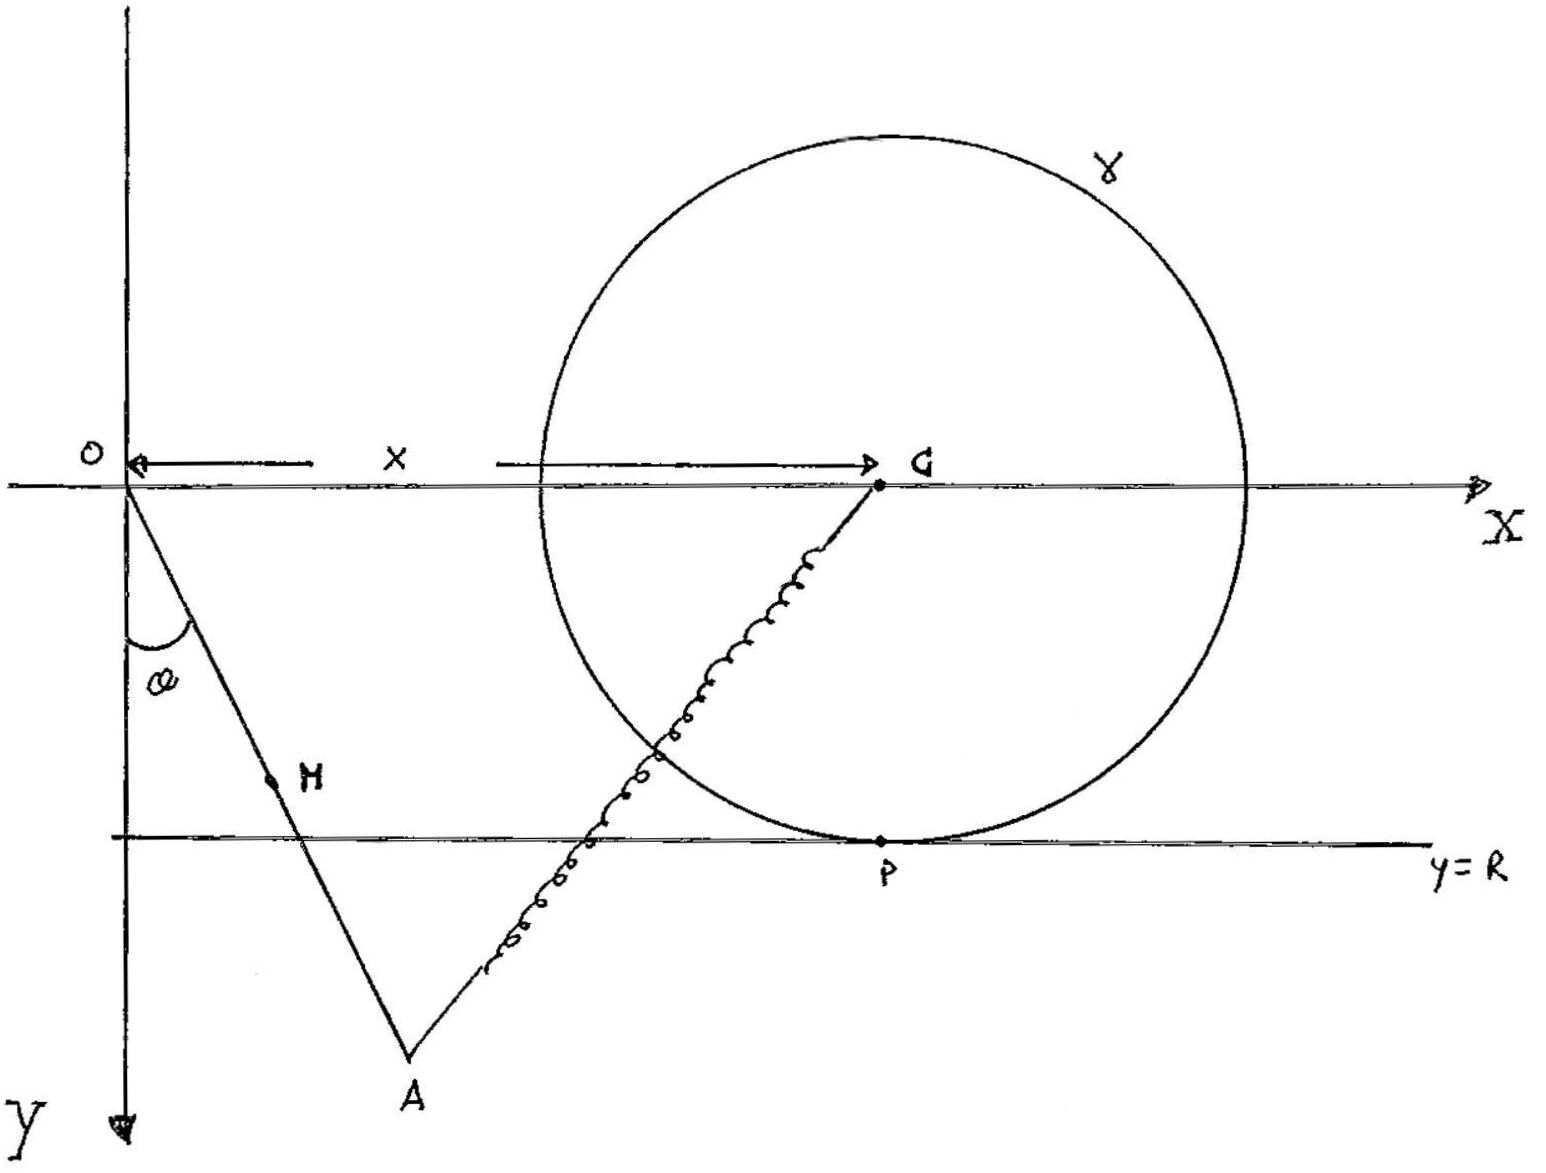
\includegraphics[max width=\textwidth]{2023_04_03_c2b519dab57738b76b16g-18}
\end{center}


\end{document}